% Template for ICASSP-2017 paper; to be used with:
%          spconf.sty  - ICASSP/ICIP LaTeX style file, and
%          IEEEbib.bst - IEEE bibliography style file.
% --------------------------------------------------------------------------

\documentclass{article}
\usepackage{spconf,amsmath,graphicx}
\usepackage{cite}
%\usepackage[cmex10]{amsmath}
\usepackage{graphics}
\usepackage{graphicx}
\usepackage{subfigure}
\usepackage{epsfig}
\usepackage{algorithmic}
\usepackage[linesnumbered,ruled,slide]{algorithm2e}
\usepackage{amsfonts}
\usepackage{float}
\usepackage{enumerate}
\usepackage{verbatim}
\usepackage{caption3}
\usepackage[justification=centering]{caption}
\usepackage{epstopdf}
\usepackage{url}
\usepackage{array,subfig}
\usepackage{bm} %%公式加粗

% Example definitions.
% --------------------
\def\x{{\mathbf x}}
\def\L{{\cal L}}

% Title.
% ------
\title{Robust Sequence-Based Localization in Acoustic Sensor Networks}
%
% Single address.
% ---------------

%\author{\IEEEauthorblockN{Naigao Jin, Lei Wang,}\\
%\IEEEauthorblockA{School of Software, Dalian University of Technology, China\\
%Key Laboratory for Ubiquitous Network and Service Software of Liaoning Province\\
%ngjin@dlut.edu.cn}
%\thanks{Naigao Jin is the corresponding author.}

\name{Naigao Jin, Xin Zhou, Zihan Wang, Yu Liu, Lei Wang \thanks{Naigao Jin is the corresponding author.}}


\address{School of Software, Dalian University of Technology,China\\
	Email: {ngjin, lei.wang} @dlut.edu.cn, zhouxin964@gmail.com, zihan.wang@gmail.com, psodream@126.com}

%\address{
%	School of Software, Dalian University of Technology\\
%	Key Laboratory for Ubiquitous Network and Service Software of Liaoning Province\\
%	Dalian,China\\
%}

%
% For example:
% ------------
%\address{School\\
%	Department\\
%	Address}
%
% Two addresses (uncomment and modify for two-address case).
% ----------------------------------------------------------
%\twoauthors
%  {A. Author-one, B. Author-two\sthanks{Thanks to XYZ agency for funding.}}
%	{School A-B\\
%	Department A-B\\
%	Address A-B}
%  {C. Author-three, D. Author-four\sthanks{The fourth author performed the work
%	while at ...}}
%	{School C-D\\
%	Department C-D\\
%	Address C-D}
%
\begin{document}
	%\ninept
	%
	\maketitle
	%
	\begin{abstract}
		
Acoustic source localization in sensor network is a challenging task because of severe constraints on cost, energy, and effective range of sensor devices.
To overcome these limitations in existing solutions, this paper formally describes, designs, implements, and evaluates a Half Plane Intersection method to Sequence-Based Localization, i.e., HPI-SBL, in distributed smartphone networks.
The localization space can be divided into distinct regions, and each region can be uniquely identified by the node sequence that represents the ranking of distances from the reference nodes to the region.
The key idea behind HPI-SBL is to turn the localization problem into half-plane intersection by processing the node sequence.
The proposed design is evaluated through extensive simulations and physical experiments in an indoor test-bed with 30 smartphone nodes.
Evaluation results show that HPI-SBL can effectively locate the acoustic source with good robustness.
	\end{abstract}
	%
	\begin{keywords}
Sequence-based localization, acoustic sensor networks, half plane intersection 
	\end{keywords}
	%
\section{Introduction}

Acoustic source localization (ASL) is an important signal processing task, and has a wide range of application scenarios, such as speaker-location-aware audio capturing in videoconferencing \cite{guo2011localising}, shooter localization in a battle field \cite{sallai2011acoustic}, and wild biological acoustic studies \cite{allen2008voxnet}. 
The traditional centralized microphone array-based solution to ASL exploited multiple synchronized microphones to simultaneously acquire multiple signals, 
which had some limitations with regard to the distances between the microphones, and sensing range for the large-scale applications.
Wireless acoustic sensor networks (WASNs) can overcome these limitations. 
A WASN consists of a set of wireless microphone nodes that are spatially distributed over the environment, usually in an ad-hoc fashion. 
Due to the wireless communication capabilities, the array-size limitations disappear and the microphone nodes can physically cover a much larger area. 

% Wang, \emph{et al.} \cite{wang2003acoustic} described a system having static cluster architecture, the system experienced a problem in that the accuracy decreased when an acoustic source occurred between the clusters.
% Chen, \emph{et al.} \cite{chen2004dynamic} showed that nodes in the system did not need to recognize their cluster head, reducing the constraints on deployment of the localization system.
% Hu, et al. \cite{hu2009design} design the system based on 2-tier architecture, which experienced cost and deployment problems especially in the very large target area.
% Rabbat, \emph{et al.} \cite{rabbat2005robust} proposed a decentralized algorithm based on the distributed ML estimation technique using token ring architecture.
% Kim, \emph{et al.} \cite{kim2009locating} proposed to identify the node closest to the acoustic source, based on TOA comparisons between all nodes, thus incurring high communication cost and requiring global synchronization between all sensor nodes.
% Lightning is a method proposed in \cite{wang2008lightning} to identify the sensor closest to the acoustic source, also based on expensive broadcasting/flooding.
Acoustic source localization problem in sensor networks has been widely studied in the literature. 
There is a trade-off between the accuracy of localization and the computational complexity for existing different solutions.
Most of localization systems are based on range information, such as distance measurements and angle measurements among sensor nodes. 
Range-based localization methods can achieve good localization performance, however, generally are sensitive to the mesurement errors\cite{zhong2009tracking}. 
%\cite{yang2013freeloc} \cite{shu2015toc}
%The requirement of low cost and power prohibits many range-based methods for acoustic source localization, especially for large-scale deployments. 
Yedavalli, \emph{et al.}~\cite{yedavalli2008sequence} proposed a range-free Sequence-Based Localization (SBL) method in wireless sensor networks. 
The heart of SBL is the division of a 2D localization space into distinct regions by the perpendicular bisectors of lines joining pairs of anchor nodes.
Each distinct region can be uniquely identified by a node sequence that represents the distance ranks of the acoustic source to that region. 
Based on the rank of measurements between the acoustic source and the sensor nodes, the location of acoustic source can be estimated by searching through the node sequence table.
%Zhong, \emph{et al.} \cite{zhong2009tracking} converted the original tracking problem to the problem of finding the shortest path in a graph, which is equivalent to optimal matching of the node sequences. 
%Zhong, \emph{et al.} \cite{zhong2011rsd} introduced a proximity metric called RSD to capture the distance relationships among 1-hop neighboring nodes in a range-free manner. With little overhead, RSD can be conveniently applied for connectivity-based localization solutions to achieve better accuracy.

In this paper, we present a robust Half Plane Intersection to Sequence-Based Localization (HPI-SBL) by deeply mining the information embedded in the node sequence. 
As a range-free scheme, our design applies node sequences instead of direct time of arrival (TOA) as the measurement information, and has the following two major advantages: 
(i) node sequences are more robust to the measurement noise; 
(ii) node sequences significantly alleviate the accuracy requirement of time synchronization in sensor networks. 
Compared with earlier works on sequence-based localization in sensor
networks (e.g. SBL~\cite{yedavalli2008sequence}), the primary contribution
of our work is providing a robust approach to solve the sequence-based localization problem with the uncertainty of node position errors and measurement errors. 
The proposed HPI-SBL system formulates the localization as the probabilistic half-plane intersection problem. 
The proposed design is evaluated with both test-bed experiments and extensive simulations. 
Evaluation results show that the proposed HPI-SBL system can provide improved localization robustness.


The rest of the article is organized as follows. Section \uppercase\expandafter{\romannumeral 2} presents the localization system model.
Then, our methods are introduced in section \uppercase\expandafter{\romannumeral 3}.
Section \uppercase\expandafter{\romannumeral 4} presents simulation results . 
Section \uppercase\expandafter{\romannumeral 5} concludes the whole article.

% The remainder of the article is organized as follows. 
% Section \uppercase\expandafter{\romannumeral 2} presents an overview of the  localization system.
% Then, the basic HPI-SBL and advanced HPI-SBL is introduced in section \uppercase\expandafter{\romannumeral 3}.
% %Section \uppercase\expandafter{\romannumeral 4} discusses several practical issues.
% Section \uppercase\expandafter{\romannumeral 5} presents simulation results and an empirical evaluation. 
% Section \uppercase\expandafter{\romannumeral 6} briefly surveys related work.
% Section \uppercase\expandafter{\romannumeral 7} concludes the article.






\section{System Model}

% ˫����ʽ�м��������ͼ��:��\begin{figure}�м���*���ɣ�����\begin{figure*}  \end{figure*} ��

\begin{figure}[htb]
  \centering
 %\setlength{\abovecaptionskip}{-15pt}
 %\setlength{\belowcaptionskip}{-5pt}
    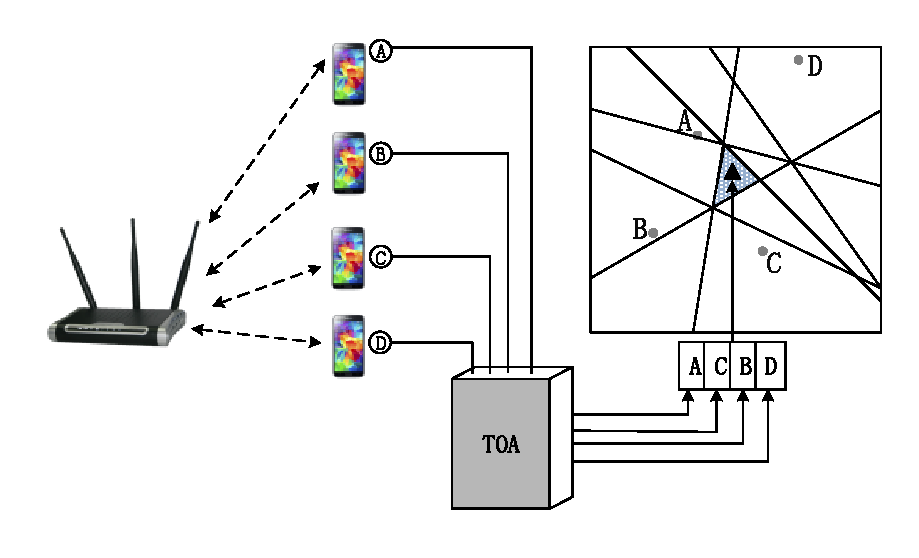
\includegraphics[height=4.5cm]{image/fig1.pdf} 
    \caption{Overview of HPI-SBL}
 \label{overview}
    \end{figure}


In this section, we focus mainly on the system overview of our HPI-SBL system, which aims at locating an acoustic source with the node sequence. 
Fig.1 shows a layout of a acoustic sensor network with $N$ sensor nodes and the acoustic source.
We use circles and the triangle to stand for sensor nodes and the acoustic source, respectively.
Consider any two reference nodes and draw a perpendicular bisector to the line joining their locations. This perpendicular bisector divides the localization
space into two different regions that are distinguished by their proximity to either reference nodes, as illustrated in Fig.1. 
Similarly, if perpendicular bisectors are drawn for all pairs of reference nodes, they can divide the localization space into many regions.
All locations inside a region have the same node sequence, and the node sequence of a given region is unique to that region.
If each region in the arrangement is represented by its centroid, then there exists a one-to-one mapping between a node sequence and the centroid of the region that it represents.

Briefly, sequence-based localization system works as follows. 
Sensor nodes detect the acoustic event sequentially at different time instances, then an order of related nodes, called node sequence, is naturally generated. 
For instance, in Fig.1, when the acoustic source generates a wave, the node sequence $NodeSeq (A C B D)$ is obtained along the sound propagation. 
The node sequence implies the location information of the acoustic source. 
By gathering the TOA measurement data from sensor nodes, the location of the acoustic source can be estimated by processing the node sequence. 

Fig.2 shows that $NodeSeq (A C B D)$ can be achieved by TOA measurement of the acoustic event.
We can get the distance sequence ${SA} < {SC} < {SB} < {SD}$ from each node to the acoustic source $S$.
$SA<SC$ shows that the acoustic source $S$ lies in the right half-plane of the perpendicular bisector of A and C.
Similarly, $SC<SB$ means that the acoustic source $S$ lies in the left half-plane of the perpendicular bisector of C and B.
$SB<SD$ shows that the acoustic source $S$ lies in the left half-plane of the perpendicular bisector of B and D.
The intersection of the three half-planes is the final region of the acoustic source.


    \begin{figure}[!htb]
    \centering
 \setlength{\abovecaptionskip}{-15pt}
                     \vspace{-3.5mm}  
 %\setlength{\belowcaptionskip}{-5pt}
    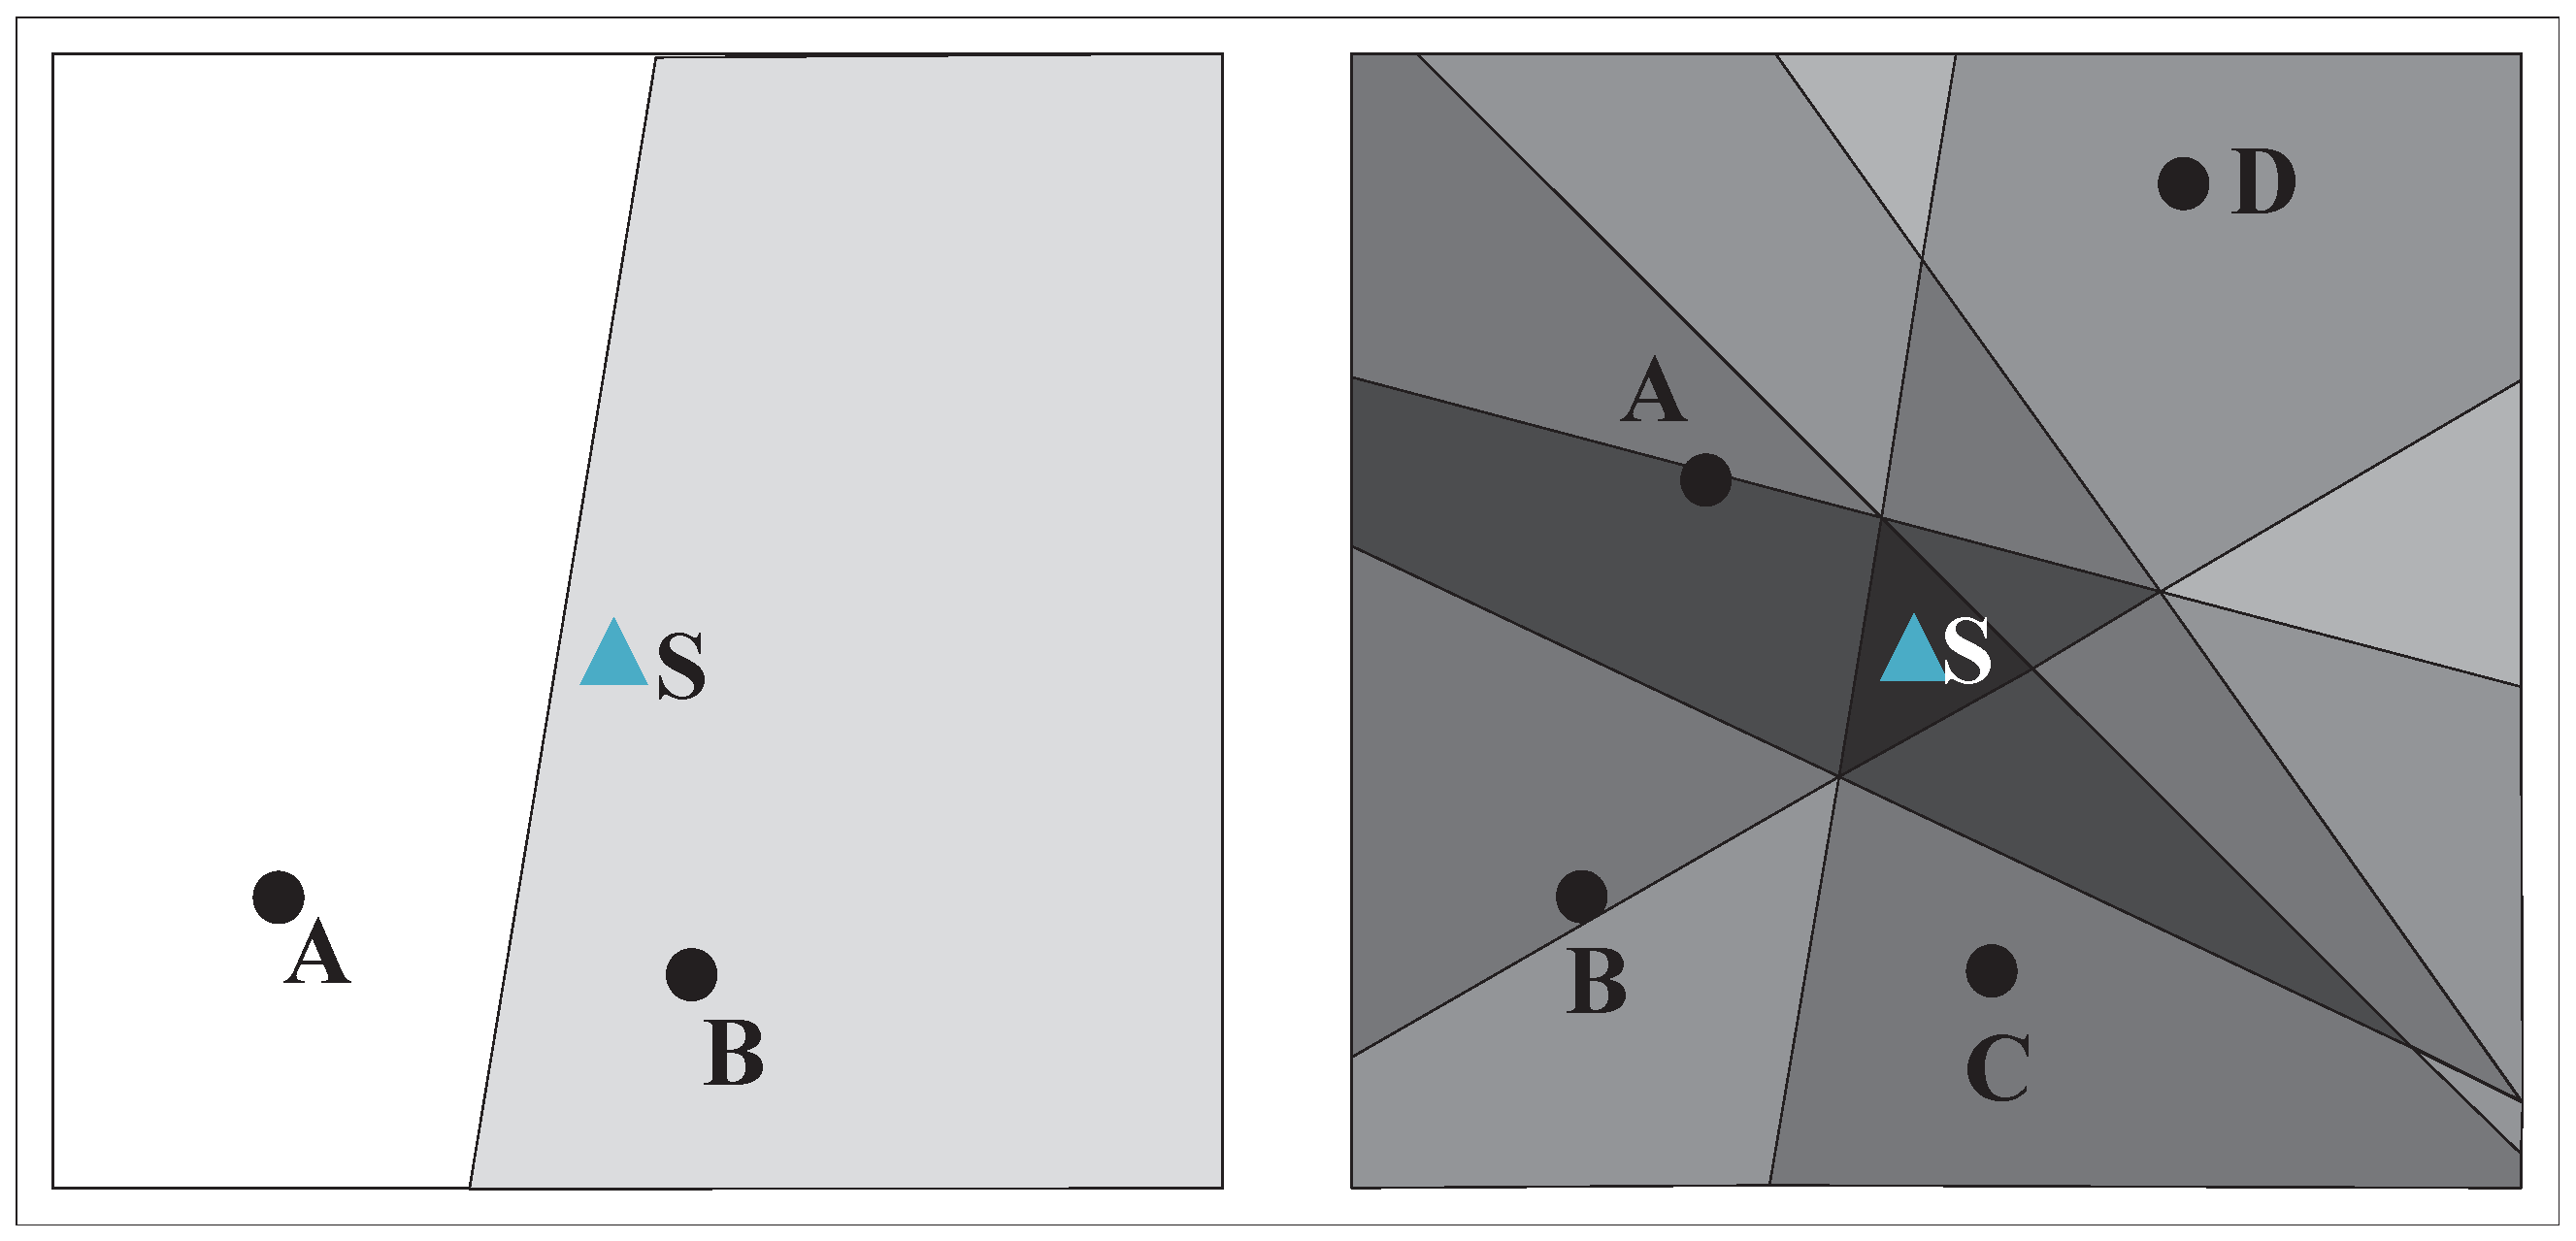
\includegraphics[height=4cm]{image/fig2.eps} 
	\vspace{10mm}
    \caption{The basic idea of HPI-SBL}
	\label{fig2}
    \vspace{-3.5mm}
    \end{figure}

	
Compared to earlier works on sequence-based localization  with brute force searching scheme (SBL~\cite{yedavalli2008sequence}), 
we carefully formulate sequence-based localization as the traditional half-plane intersection problem. 
To the best of our knowledge, this is the first work to leverage half-plane intersection for solving sequence-based localization problems in sensor networks.








\section{DESIGN}

In this section, we firstly introduce the basic HPI-SBL method.
After the basic HPI-SBL method is proposed, we describe the probabilistic HPI-SBL method in the next subsection. Finally, weighted probabilistic HPI-SBL, the robust version of HPI-SBL is given.
%Finally, the computational complexity analysis of HPI-SBL is given.

\subsection{Basic HPI-SBL }

In this section, we introduce the basic sequence-based localization technique based on half-plane intersection.

Considering a sensor network in the 2D space with $N$ nodes, all nodes are $\bm{X} = \{ \bm{nod{e_1}}, \cdots ,\bm{nod{e_i}}, \cdots ,\bm{nod{e_N}}\}$, 
where any node $\bm{nod{e_i}}$ has its location coordinate denoted as $[{x_i},{y_i}]$. 
As showed in Fig. 2, an acoustic event occurs at $\bm{X_s}{\rm{ = [}}{x_s},{y_s}]$, ${d_i}$ is the distance from $\bm{nod{e_i}}$ to the acoustic source $\bm{S}$.
The node sequence is determined by the distances from nodes to the acoustic source $\bm{S}$.

Basic HPI-SBL turns the localization problem into half-plane intersection by processing the node sequence. 
The half-planes are constructed by the two adjacent nodes in the node sequences. 
We can find a solution to narrow the source region by making intersection of these half-planes. 
Given the following node sequence $NodeSeq( \cdots ,i,j,k,\cdots )$  obtained by time of arrival (TOA) information of the acoustic event,
we can get the distance sequence ${d_i} < {d_j} < {d_k} $ from  the acoustic source  to each node.
Just considering the adjacent node, we can have the following $N(N-1)/2$ linear constraints: $d_i<d_j$, $d_i<d_k$ and $d_j<d_k$, etc. 
We construct the corresponding $N(N-1)/2$  half-planes $H_{ij}$, $H_{ik}$ and $H_{jk}$, etc.
$d_i<d_j$ means that the acoustic source lies in the left half-plane $H_{ij}$ of the perpendicular bisector of $\bm{nod{e_i}}$ and $\bm{nod{e_j}}$.
The intersection of  the $N(N-1)/2$  half-planes is the final region of the acoustic source.
% \begin{algorithm}
% \caption{Basic HPI-SBL}
% \KwIn { The location of $N$ smartphones \\
% \hspace{0.41in} The node sequence of the acoustic source for\\
% \hspace{0.41in} $N$ reference nodes
% }
% \KwOut {Location of the acoustic source}

% \textbf{Step 1:} Setting the original region $R_S$ of acoustic source $S$: $R_S \leftarrow The whole space$;

% \textbf{Step 2:} Narrow the region by half-plane intersection: \\ 
% \hspace{0.41in} setting $\bm{A}$ and $\bm{b}$ by processing node sequence;\\
% \For{$i \leftarrow 1$ \textbf{to} $N-1$}
% {
% \For{$j \leftarrow i+1$ \textbf{to} $N$}
% {
% Use $node_i$ and $node_j$ to contruct half-plane $H_{ij}$;

% Solve half-plane intersection problem to get the target's location.

% $R_S$= $R_S$ U $H_{ij}$
% }
% }
% \textbf{Step 3:} the center of region $R_S$ is the target's location.
% \end{algorithm}

\subsection{Probabilistic HPI-SBL}

For the sake of presentation, until now we have described HPI-SBL in an ideal case where a complete and perfect node sequence can be obtained. 
In this section, we describe how to make HPI-SBL work well under more realistic conditions. 

%Basic HPI-SBL can find a solution to this feasibility program only if there is a region satisfying all the constraints. 
In the practical application, if two nodes are very close to each other along the direction of event propagation, they would detect the event almost simultaneously. 
In this case, the flip problem of node sequence may occur. 
%For instance, the true sequence is $NodeSeq ( \cdots ,i,j, \cdots )$, but the detected sequence is $NodeSeq ( \cdots ,j,i, \cdots )$.
Basic HPI-SBL might fail to find a feasible solution that satisfies all the constraints when sequence flip occurs. 
For example, as shown in Fig.2, the right middle region identifies by the node sequence $NodeSeq (D B C A)$. 
Once the order of node A and C is flipped in $NodeSeq (D B C A)$, the region corresponding to $NodeSeq (D B A C)$  does not exist, basic HPI-SBL can not give the accurate estimation.
In this section, we propose a robust solution to address the problem of sequence flip, called probabilistic HPI-SBL.

Considering the uncertainty of the measurement with the node sequence $NodeSeq( \cdots ,i,j, \cdots )$, the probability of ${d_i} < {d_j}$ can be described as  
 \begin{equation}\label{eqq1}
 p({d_i} < {d_j})>\alpha
 \end{equation}
Eq.\ref{eqq1} means that the probability of the acoustic source in the left side of the the half-plane $H_{ij}$ is $\alpha$, and the right side is $1-\alpha$. 
After dividing the localization space into some discrete grids, the weight of the grid point in the left side of the the half-plane $H_{ij}$ is $\alpha$, and the weight of the grid point in the right side of the the half-plane $H_{ij}$ is $1-\alpha$.

Besides these key constraints mentioned in basic HPI-SBL, some relaxed constraints are also provided some localization information.
For example, given $NodeSeq (A C B D)$, three key constraints $SA<SC$, $SC<SB$ and $SB<SD$ from the two adjacent nodes,
and three relaxed constraints $SA<SB$, $SA<SD$ and $SC<SD$ from the two nonadjacent nodes in the node sequence are achieved, respectively. 
Given the node sequences with $N$ nodes, all  $N(N - 1)/2$  constraints can be ultilized to further improve the localization robustness.
By processing  $N(N - 1)/2$ half-planes, we can compute the cumulative weight $w$ of each grid point $\bm{x}$

\begin{equation}\label{eq2}
w(\bm{x})=\sum\limits_{k=1} ^{N-1}\alpha(k).
\end{equation}
The region with the highest probability is the final region of the acoustic source
\begin{equation}\label{eq3}
\hat{\bm{X_s}}=arg \max_{\bm{x} \in R}w(\bm{x}).
\end{equation}
The centroid of the final region is the estimated location of the acoustic source.


%To summarize, the probabilistic HPI-SBL is presented in Algorithm 1. 
%The input are the node sequences and anchor locations; the output is the location of the acoustic source. 
%Step 1 sets the the initial weight of each discrete grid point. 
%Step 2 uses the node sequence to get multiple half-planes, then computes the cumulative weight.
%Step 3 adopts the center of the final intersection region as the location of acoustic source.

%\begin{algorithm}
%\caption{Probabilistic HPI-SBL}
%\KwIn { The location of $N$ smartphones \\
%\hspace{0.41in} The node sequence of the acoustic source for\\
%\hspace{0.41in} $N$ smartphones
%}
%\KwOut {Location of the acoustic source}

%\textbf{Step 1:} Setting the weight of each grid point  $w(k) \leftarrow 0$;

%\textbf{Step 2:} Computing the cumulative weight by processing node sequence: \\ 
%\hspace{0.0in} Contructing half planes by processing node sequence;\\
%\For{$i \leftarrow 1$ \textbf{to} $N-1$}
%{
%\For{$j \leftarrow i+1$ \textbf{to} $N$}
%{
%Calculating the probality of the line by the distance of $i,j$\\
%Contructing half plane $H_{ij}$\\
%Updating Weight $w(k)$ by the new probability for each grid point;\\
%}
%}
%\textbf{Step 3:} The center of region with the highest probability is the location of acoustic source.
%\end{algorithm}


\subsection{Weighted Probabilistic HPI-SBL}

 Considering the uncertainty of the measurement with the node sequence $NodeSeq( 1,\cdots ,i,j, \cdots,n )$, the probability of ${d_i} < {d_j}$ can be described as  
 \begin{equation}\label{eq1}
 p({d_i} < {d_j})>\alpha_{ij}
 \end{equation}

 In real condition, we consider the probabilities given by different half-plane exist differences. Here we call the line which divide the space as edge. We believe the edge constructed by $i,j$, if closer to the acoustic source, the half-plane divided by it is more essential to localization for determining a more accurate area, meawhile, is more likely to occur flip, we give $\alpha_{ij}$ a smaller value. As for the edges further to the source, its function is inferior in localization, but impossible to occur flip so more believable, we set $\alpha_{ij}$ a large value. In this way, utilizing the weighted probability to determine the acoustic source.
 
As the node sequence $NodeSeq( \cdots ,i,j, \cdots )$ is known to us, for every half-plane, the probability change dynamically according to the distance of the edge to the acoustic source. If the node $i,j$ that construct the half-plane in the sequence is 1 and $n$, as the relative distance is the largest, we set $\alpha_{ij}$ a largest value $\alpha$, if the relative distance of $i,j$ in the sequence is the smallest 1, we give $\alpha_{ij}$ a smallest probability $\beta$. As for other half-planes, we utilize the arithmetic propression between $\alpha$ and $\beta$ by the relative distance of $i,j$ to set their probabilities.

% \begin{algorithm}
% 	\caption{Weighted Probabilistic HPI-SBL}
% 	\KwIn { The location of $N$ smartphones \\
% 		\hspace{0.41in} The largest probability $\alpha$\\
% 		\hspace{0.41in} The smallest probability $\beta$\\
% 		\hspace{0.41in} The node sequence of the acoustic source for\\
% 		\hspace{0.41in} $N$ smartphones
% 	}
% 	\KwOut {Location of the acoustic source}
% 	
% 	\textbf{Step 1:} Setting the weight of each grid point  $w(k) \leftarrow 0$;
% 	
% 	\textbf{Step 2:} Giving half-plane probabilities and computing the cumulative weight by processing node sequence: \\ 
% 	\hspace{0.0in} Contructing half planes by processing node sequence;\\
% 	\For{$i \leftarrow 1$ \textbf{to} $N-1$}
% 	{
% 		\For{$j \leftarrow i+1$ \textbf{to} $N$}
% 		{
% 			Contructing half plane $H_{ij}$\\
% 			Calculating $\alpha_{ij}$ between $\alpha$ and $\beta$ according to the relative distance of $i,j$\\
% 			Updating Weight $w(k)$ for each grid point;\\
% 		}
% 	}
% 	\textbf{Step 3:} The center of region with the highest probability is the location of acoustic source.
% \end{algorithm}

\iffalse
 \subsection{Complexity Analysis}
 This section provides the complexity analysis for the proposed
 LPSBL design. It needs to be emphasized that
 LPSBL itself adopts an asymmetric design in which sensor
 nodes need only to detect and report the events. Therefore,
 we only analyze the computational cost on the node sequence
 processing side, where resources are plentiful.

 SBL: Calculating the Spearman’s coefficient and Kendall’s Tau
 between two sequences are $O(N)$ and $O(N^2)$ operations,
 respectively. Since the location sequence table is of size
 $O(N^4)$, searching through it takes $O(N^5)$ and $O(N^6)$ operations,
 respectively~\cite{yedavalli2008sequence}.

 RSBL: Discrete space grid  M  
\fi



%\section{Discussion}

\subsection{Time Synchronization }

Like the effect of TOA detection error, time synchronization error maybe also occur flip problem when computing the node sequence in LPSBL system, then lead to localization error.
Traditional time synchronization protocol, such as RBS, TPSN, and FTSP, can achieve synchronization less than 100ns. 
Compared with the the effect of TOA detection error, time synchronization error has little effect on the LPSBL system.

\subsection{Multiple Source Localization}

Localizing multiple, simultaneously active sources is a more difficult problem. 
In order to avoid conflict of several source, multiple source localization must be able to uniquely identify the signature of each acoustic source, which is beyond the capability of this paper. 
So we will not do too much discussion about it in this paper.
We just take an example, if the several targets are set as shown in Fig. 3, then we can calculate the location of the targets 
because the acoustic source I is far enough from source II and the single from them can be distinguished. 
So the smartphones close to effective area I could handle source I, and another smartphones close to effective area II could handle source II. 
The Fig. 3 also describes system scalability.
We can use a range to divide the large-scale area into to a smaller area that is large enough to cover the coverage of the acoustic source's signal.
And the small area can be handled as our algorithm proposed by preceding part of the paper.

%  \label必须放在\caption命令的后面
  \begin{figure}[ht]
            \setlength{\abovecaptionskip}{0pt}
            \centering
            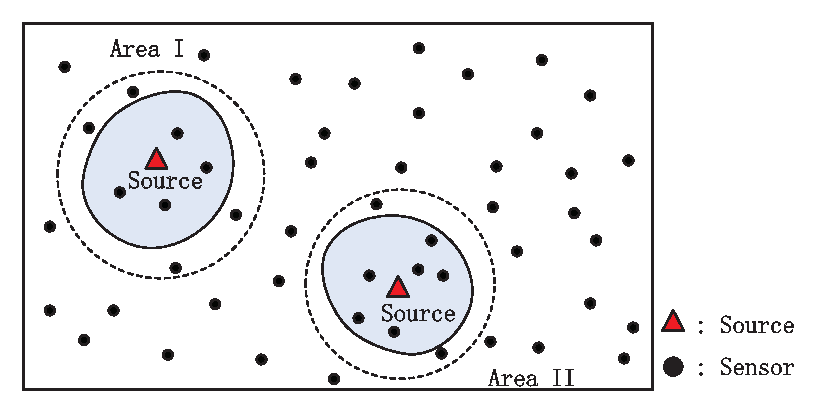
\includegraphics[scale=1.4,height=4.0cm]{image/fig3.eps}
             \vspace{1mm}
			\caption{Scalability for large-scale system}
			\label{Fig3}
            \label{multiple_source_localization}
            \vspace{-5mm}
  \end{figure}


\subsection{Energy Efficiency}

Energy efficiency is another issue in distributed acoustic sensor networks.
Most of the time, acoustic sensor nodes keep asleep until the acoustic source appears in its sensing area.  
The smartphones node near the acoustic source detect the acoustic signal, then alert its neighbour smartphones to prepare for receiving the signal.
In this way, the proposed LPSBL system can save energy of acoustic sensors, then prolong the service life of distributed acoustic sensor networks.








\section{EVALUATION }
\label{section:results}

\subsection{Simulation}
To verify our method and obtain an intuitive understanding of the localization performance under different conditions,
we developed a Monte Carlo simulator that implements
both SBL and HPI-SBL using MATLAB. 
In the simulation, we randomly deployed some smartphones (default 20) in a $10m \times 10m$ area. 
Considering the impact of the uncertainty of node position and TOA detection, we added a certain amount of node location error (default 0.4m) and TOA measurement error (default 2ms) in all the simulations.
Table 1 lists default configurations of major parameters in the simulation.
All statistics reported are RMSE  over 100 trial runs for high confidence. The results of simulation evaluation are as follows.


\begin{table} \normalsize
\caption {\textbf{Default configuration parameter}} %title of the table
\centering % centering table
    \begin{tabular}{|c|c|}
        \hline
\textbf{Parameter} & \textbf{Description} \\
 \hline
Field Area & 10m $\times$10m \\
\hline
Number of Anchors & 20 (Default) \\
 \hline
Node Location Error 	 & 0.4m (Default) \\
 \hline
TOA Detection Error 	 & 2ms (Default) \\
 \hline
Random-Seed Loop	 & 500 times (Default) \\
% \hline
%Error Statistics	 &  RMSE \\
        \hline
    \end{tabular}
\end{table}


\textbf{1) Impact of the number of anchors:}
 In this experiment, we investigated the localization error and number of anchors with a different number of anchors from 10 to 40 in steps of 3. 
 TOA error is 2ms, and other simulation parameters are default values.
With more anchors, the whole space area will be divided into smaller parts, thus more accurate localization estimation could be achieved. 
The results shown in Fig.\ref{fig4} indicates that, as the number of anchor nodes increases, the localization error decreases for both methods.
Fig.\ref{fig4} shows that the localization error of HPI-SBL method is smaller than the SBL method.

 \begin{figure}[htb]
            \setlength{\abovecaptionskip}{0pt}
            \centering
			 \vspace{-2mm}
           		 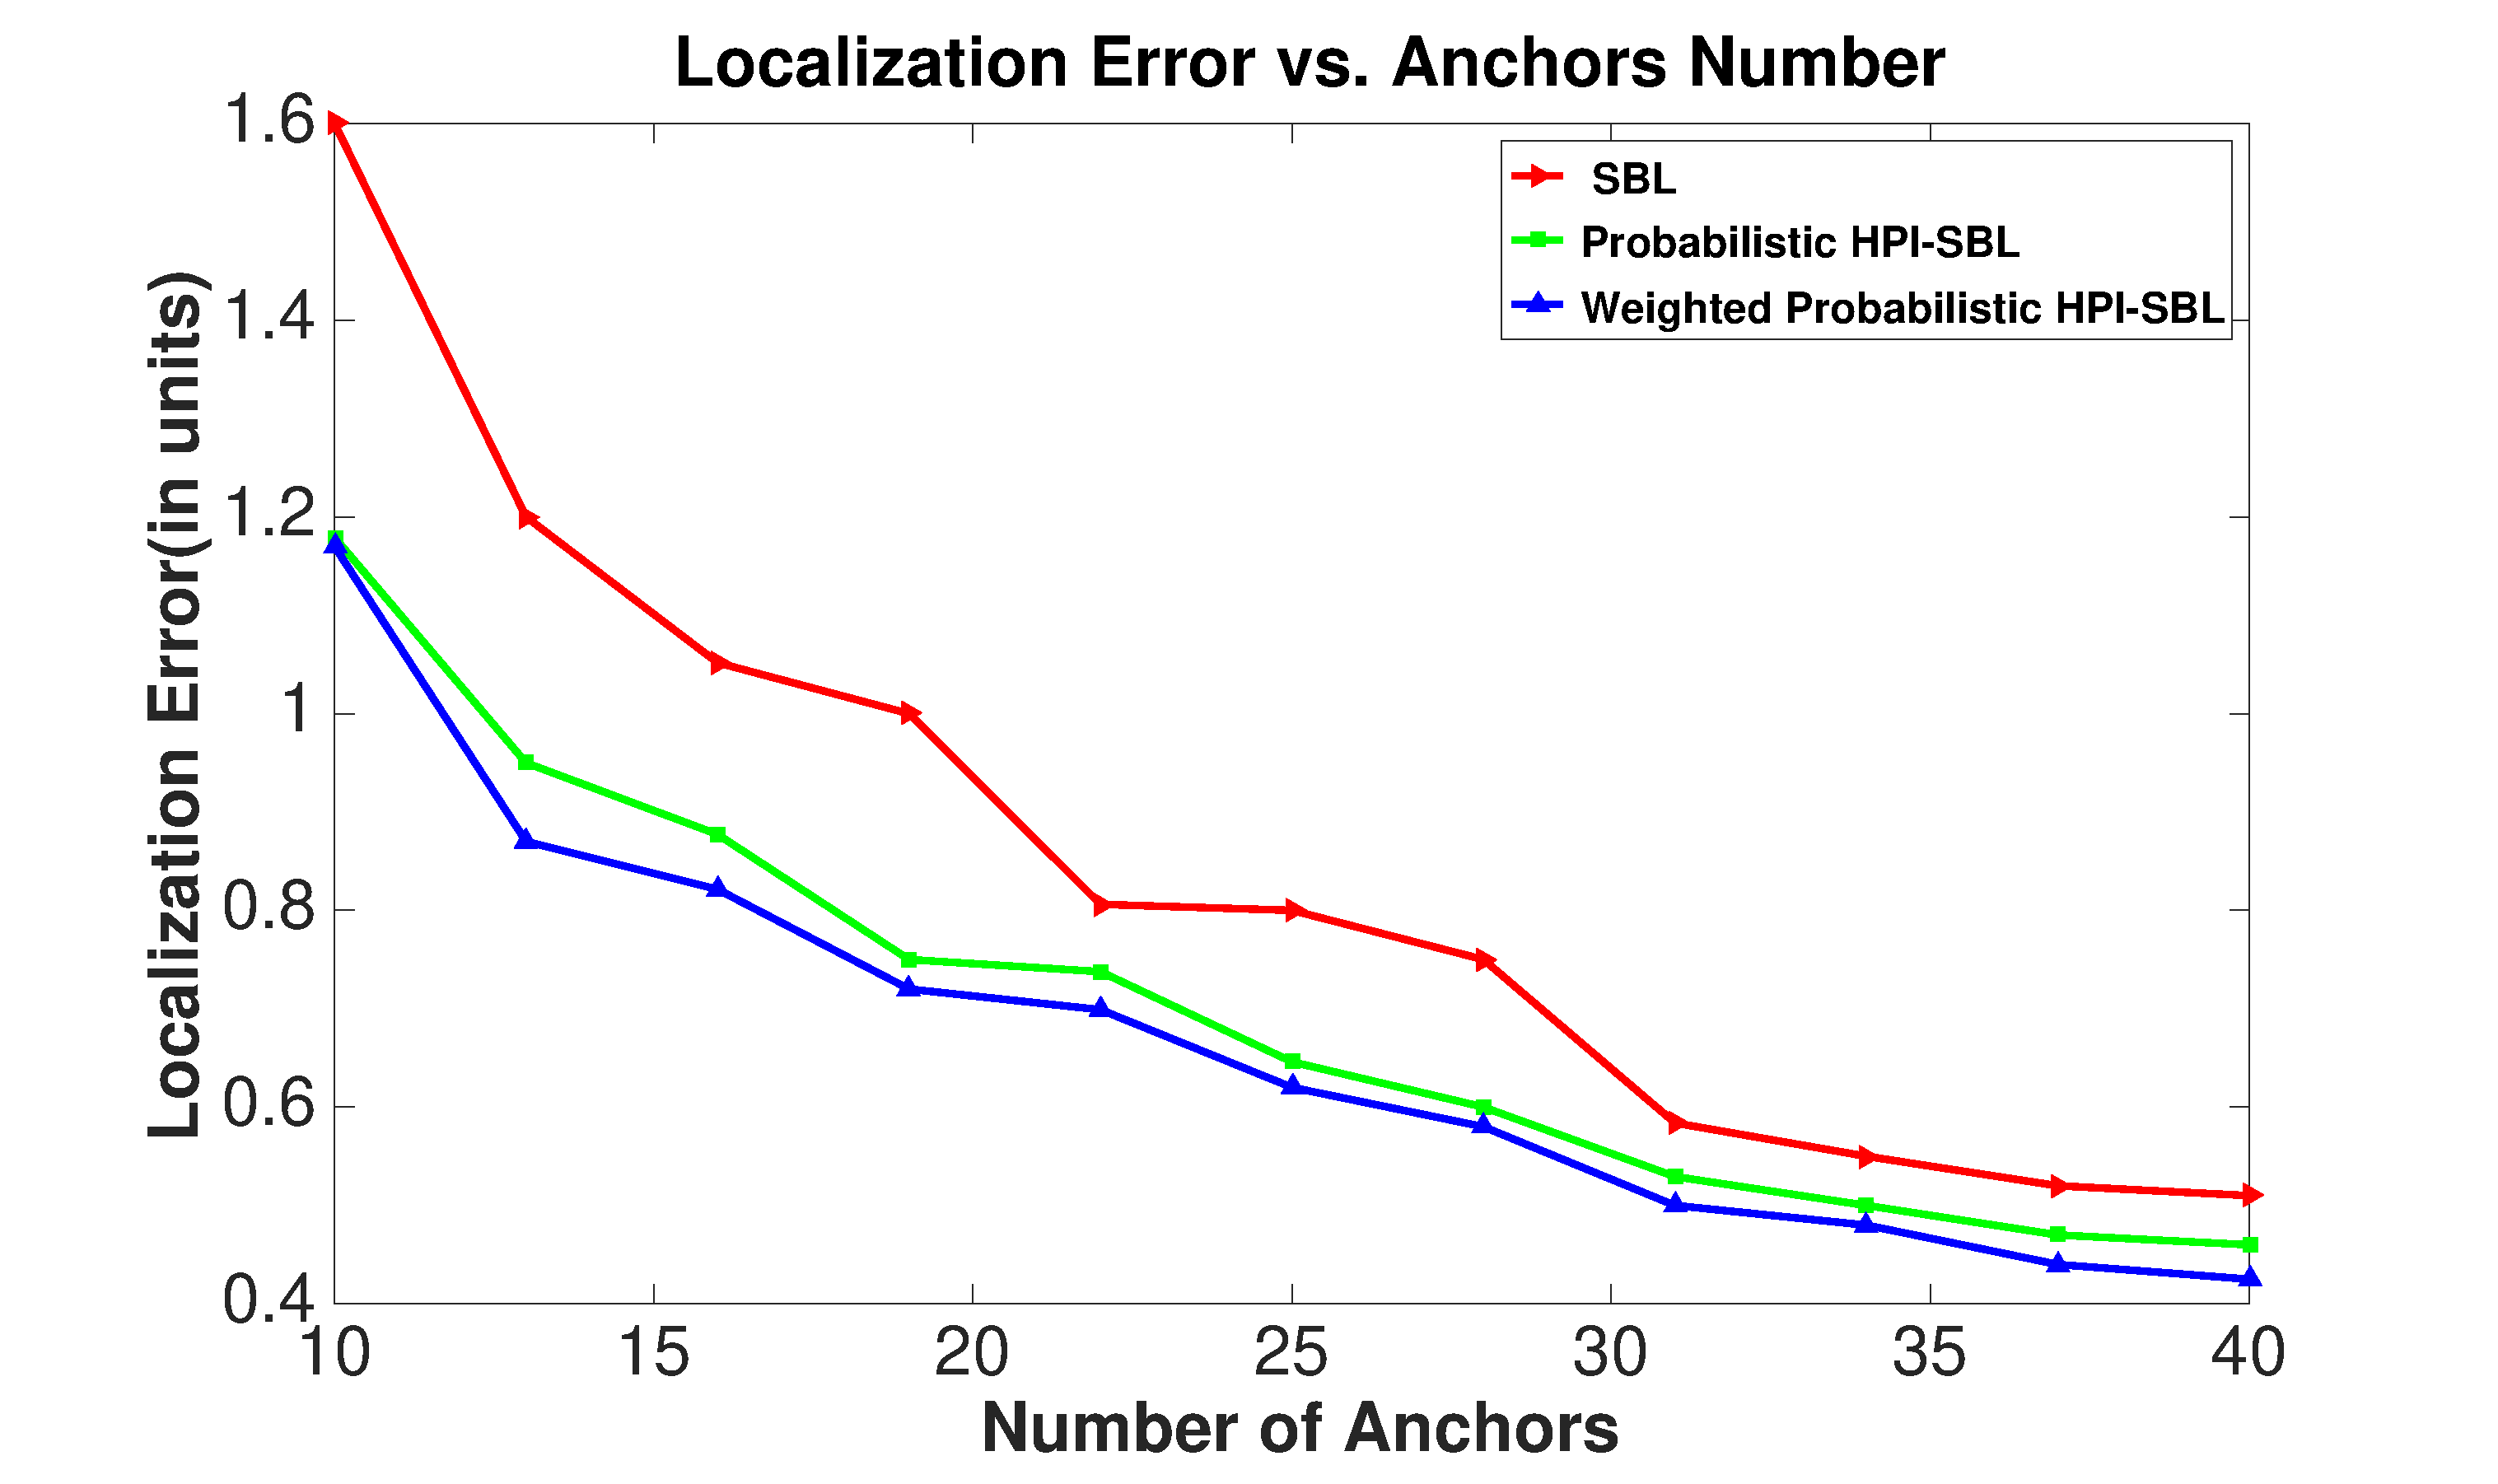
\includegraphics[height=5.0cm,width=7.0cm]{image/nodenumber.eps}
            \caption{Localization Error vs. Number of Anchors}
             \vspace{-5mm}
             \label{fig4}
        \end{figure}

		
\textbf{2) Impact of the location error:}
 %In this experiment, we compared the two methods with different location errors of anchors. 
 We choosed the location error with the range from 0 to 1m in steps of 0.05m for the three methods. 
Fig.\ref{fig5} illustrates a comparison of localization errors between the  SBL and the proposed HPI-SBL.
 Fig.\ref{fig5} indicates the location error of anchors has an effect on the localization results. 
 The proposed HPI-SBL method is more accurate than the SBL method. 
 For the SBL method, the localization error changes obviously as location error increases in Fig.\ref{fig5}. 
 However, as demonstrated in Fig.\ref{fig5}, with the increase location error of nodes, the localization error of HPI-SBL increases relatively slowly, which demonstrates the HPI-SBL method is more robust to the node location error.


  \begin{figure}[htb]
            \centering
		   \vspace{-2mm}
			 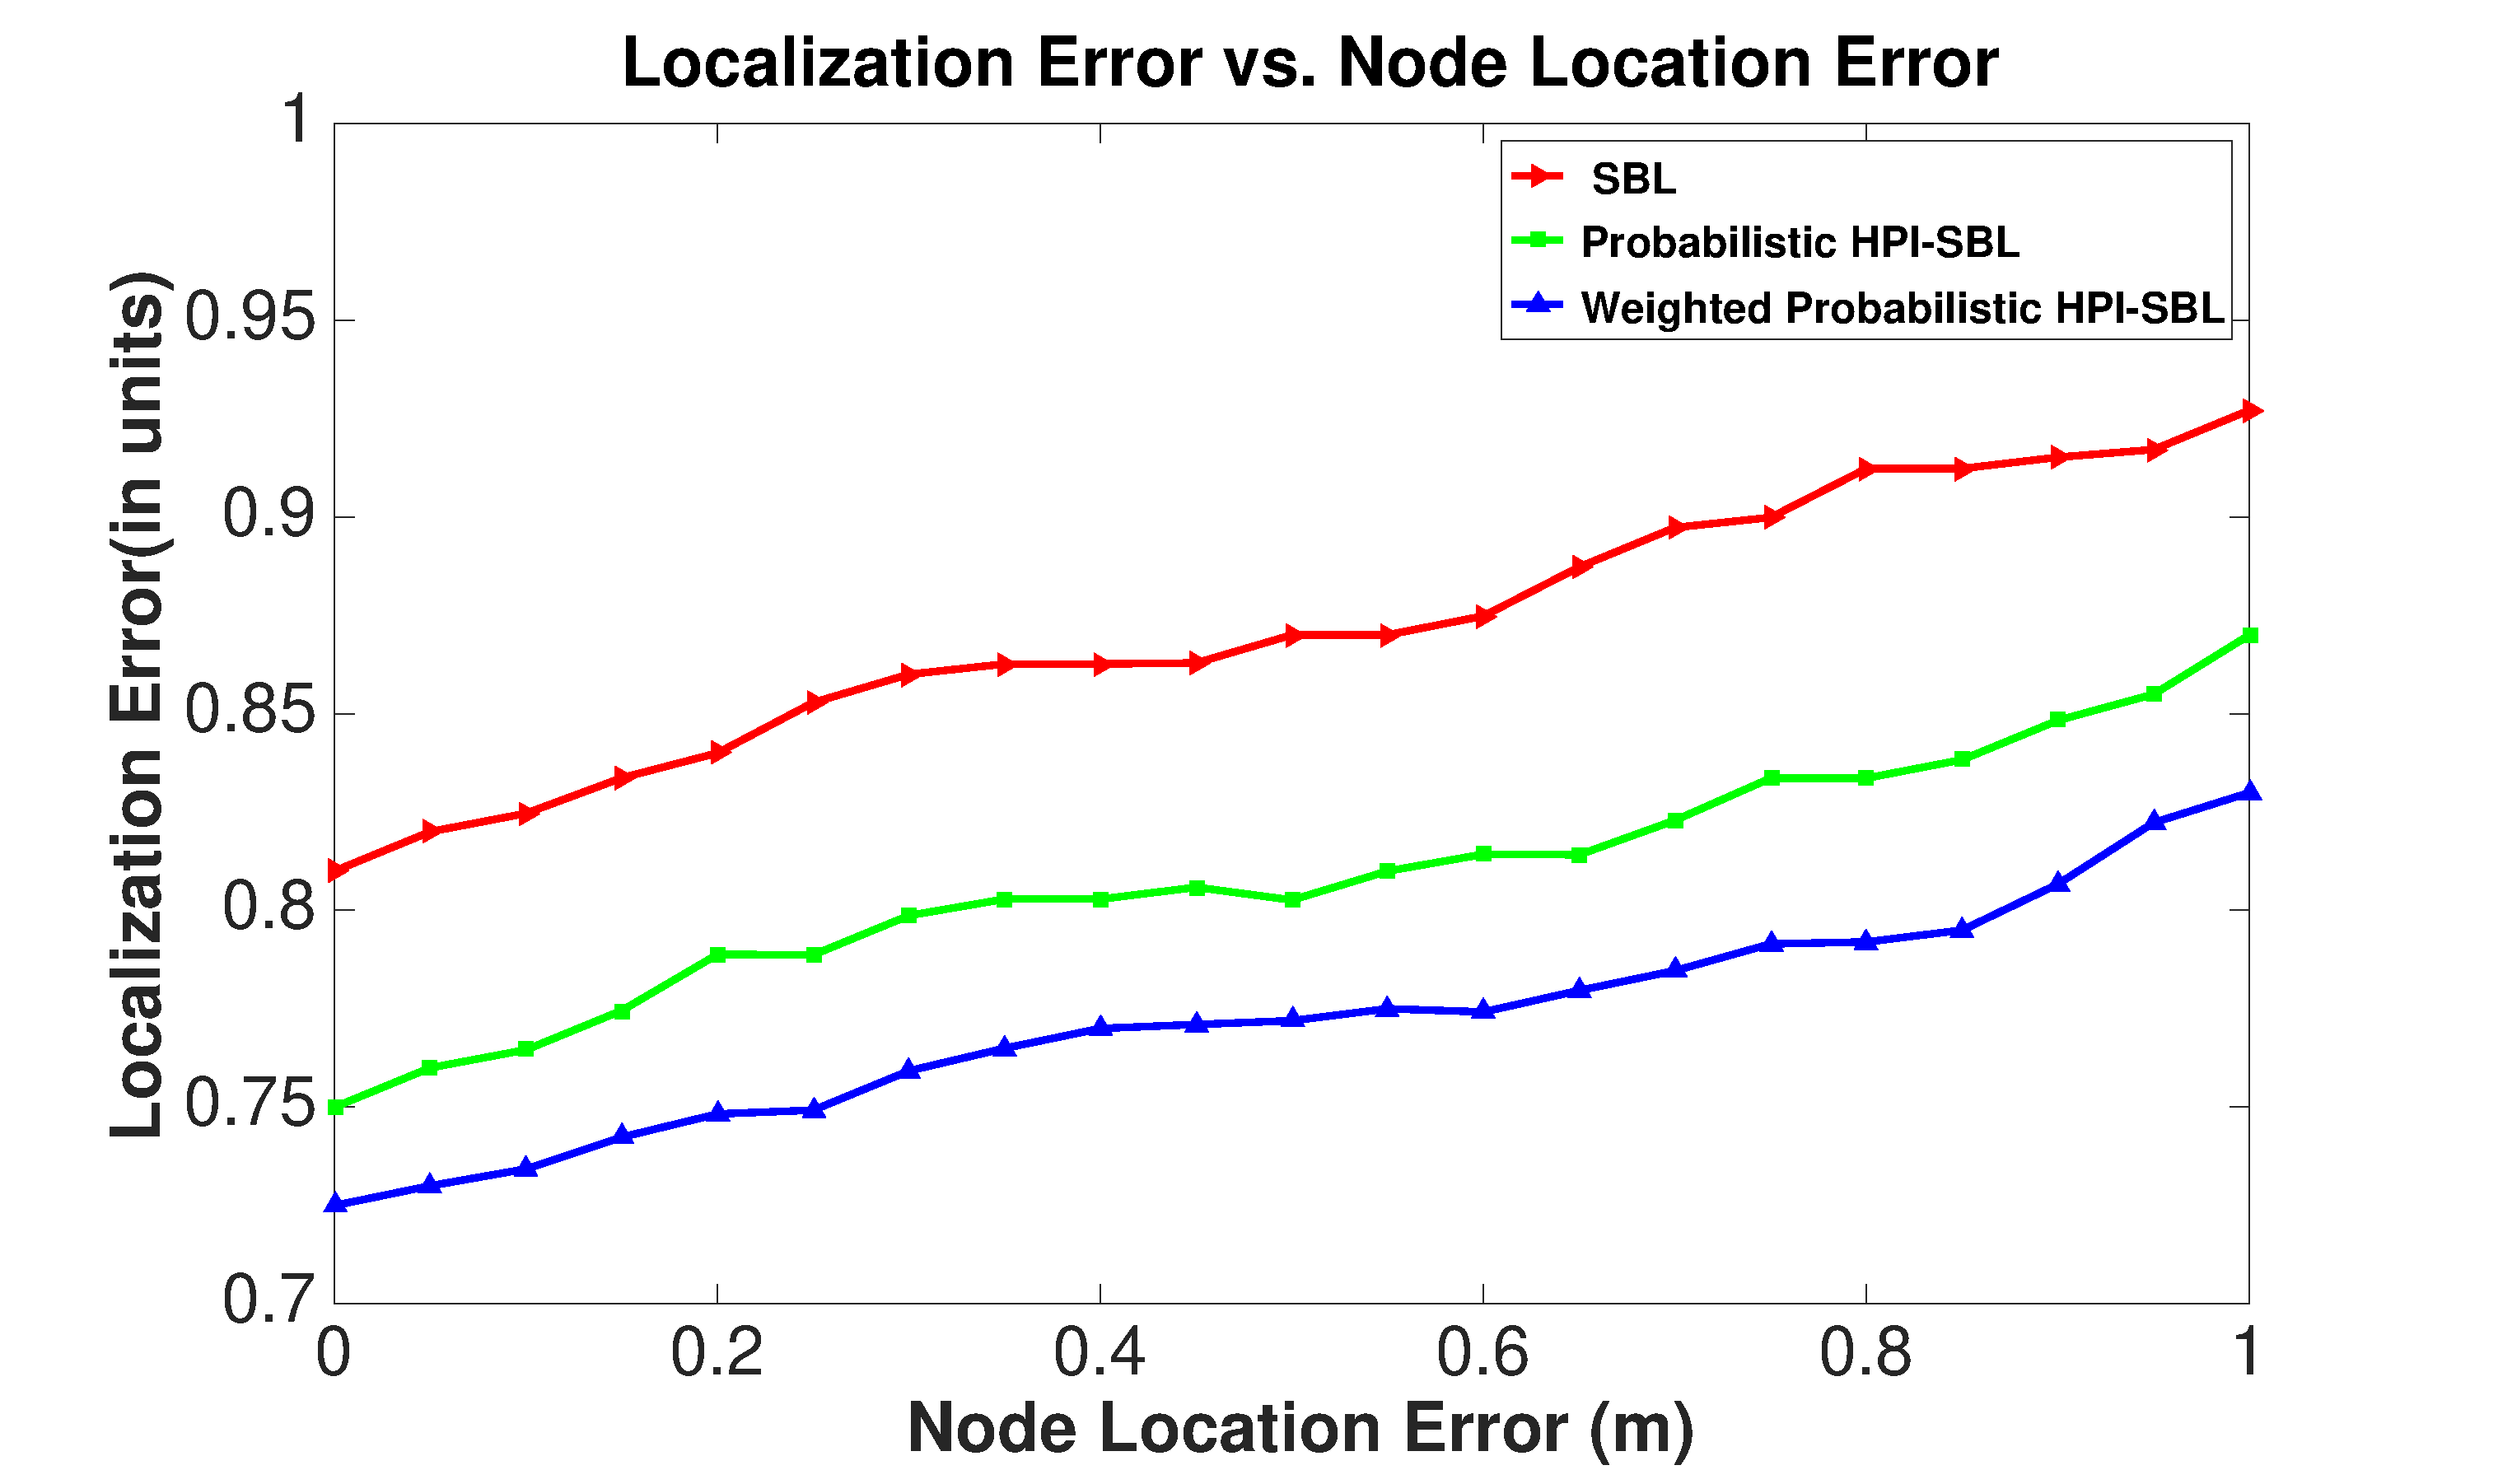
\includegraphics[height=5.0cm,width=7.0cm]{image/location.eps}
            \caption{Localization Error vs. Node Location Error}
             \vspace{-5mm}
             \label{fig5}
        \end{figure}
	

\textbf{3) Impact of the TOA measurement error:}
In this experiment, we performed the impact of the TOA error of anchors for the two methods with the range from 0 to 4ms in steps of 0.25ms. 
Other simulation parameters keep default. 
As it is shown in Fig.\ref{fig6}, the localization errors of the three methods are increasing as the TOA error growth. 
Also, the HPI-SBL method has a better result than the SBL method. We can conclude from this figure that HPI-SBL is more robust to TOA measurement error than SBL.

  \begin{figure}[htb]       
            \centering
			\vspace{-2mm}
            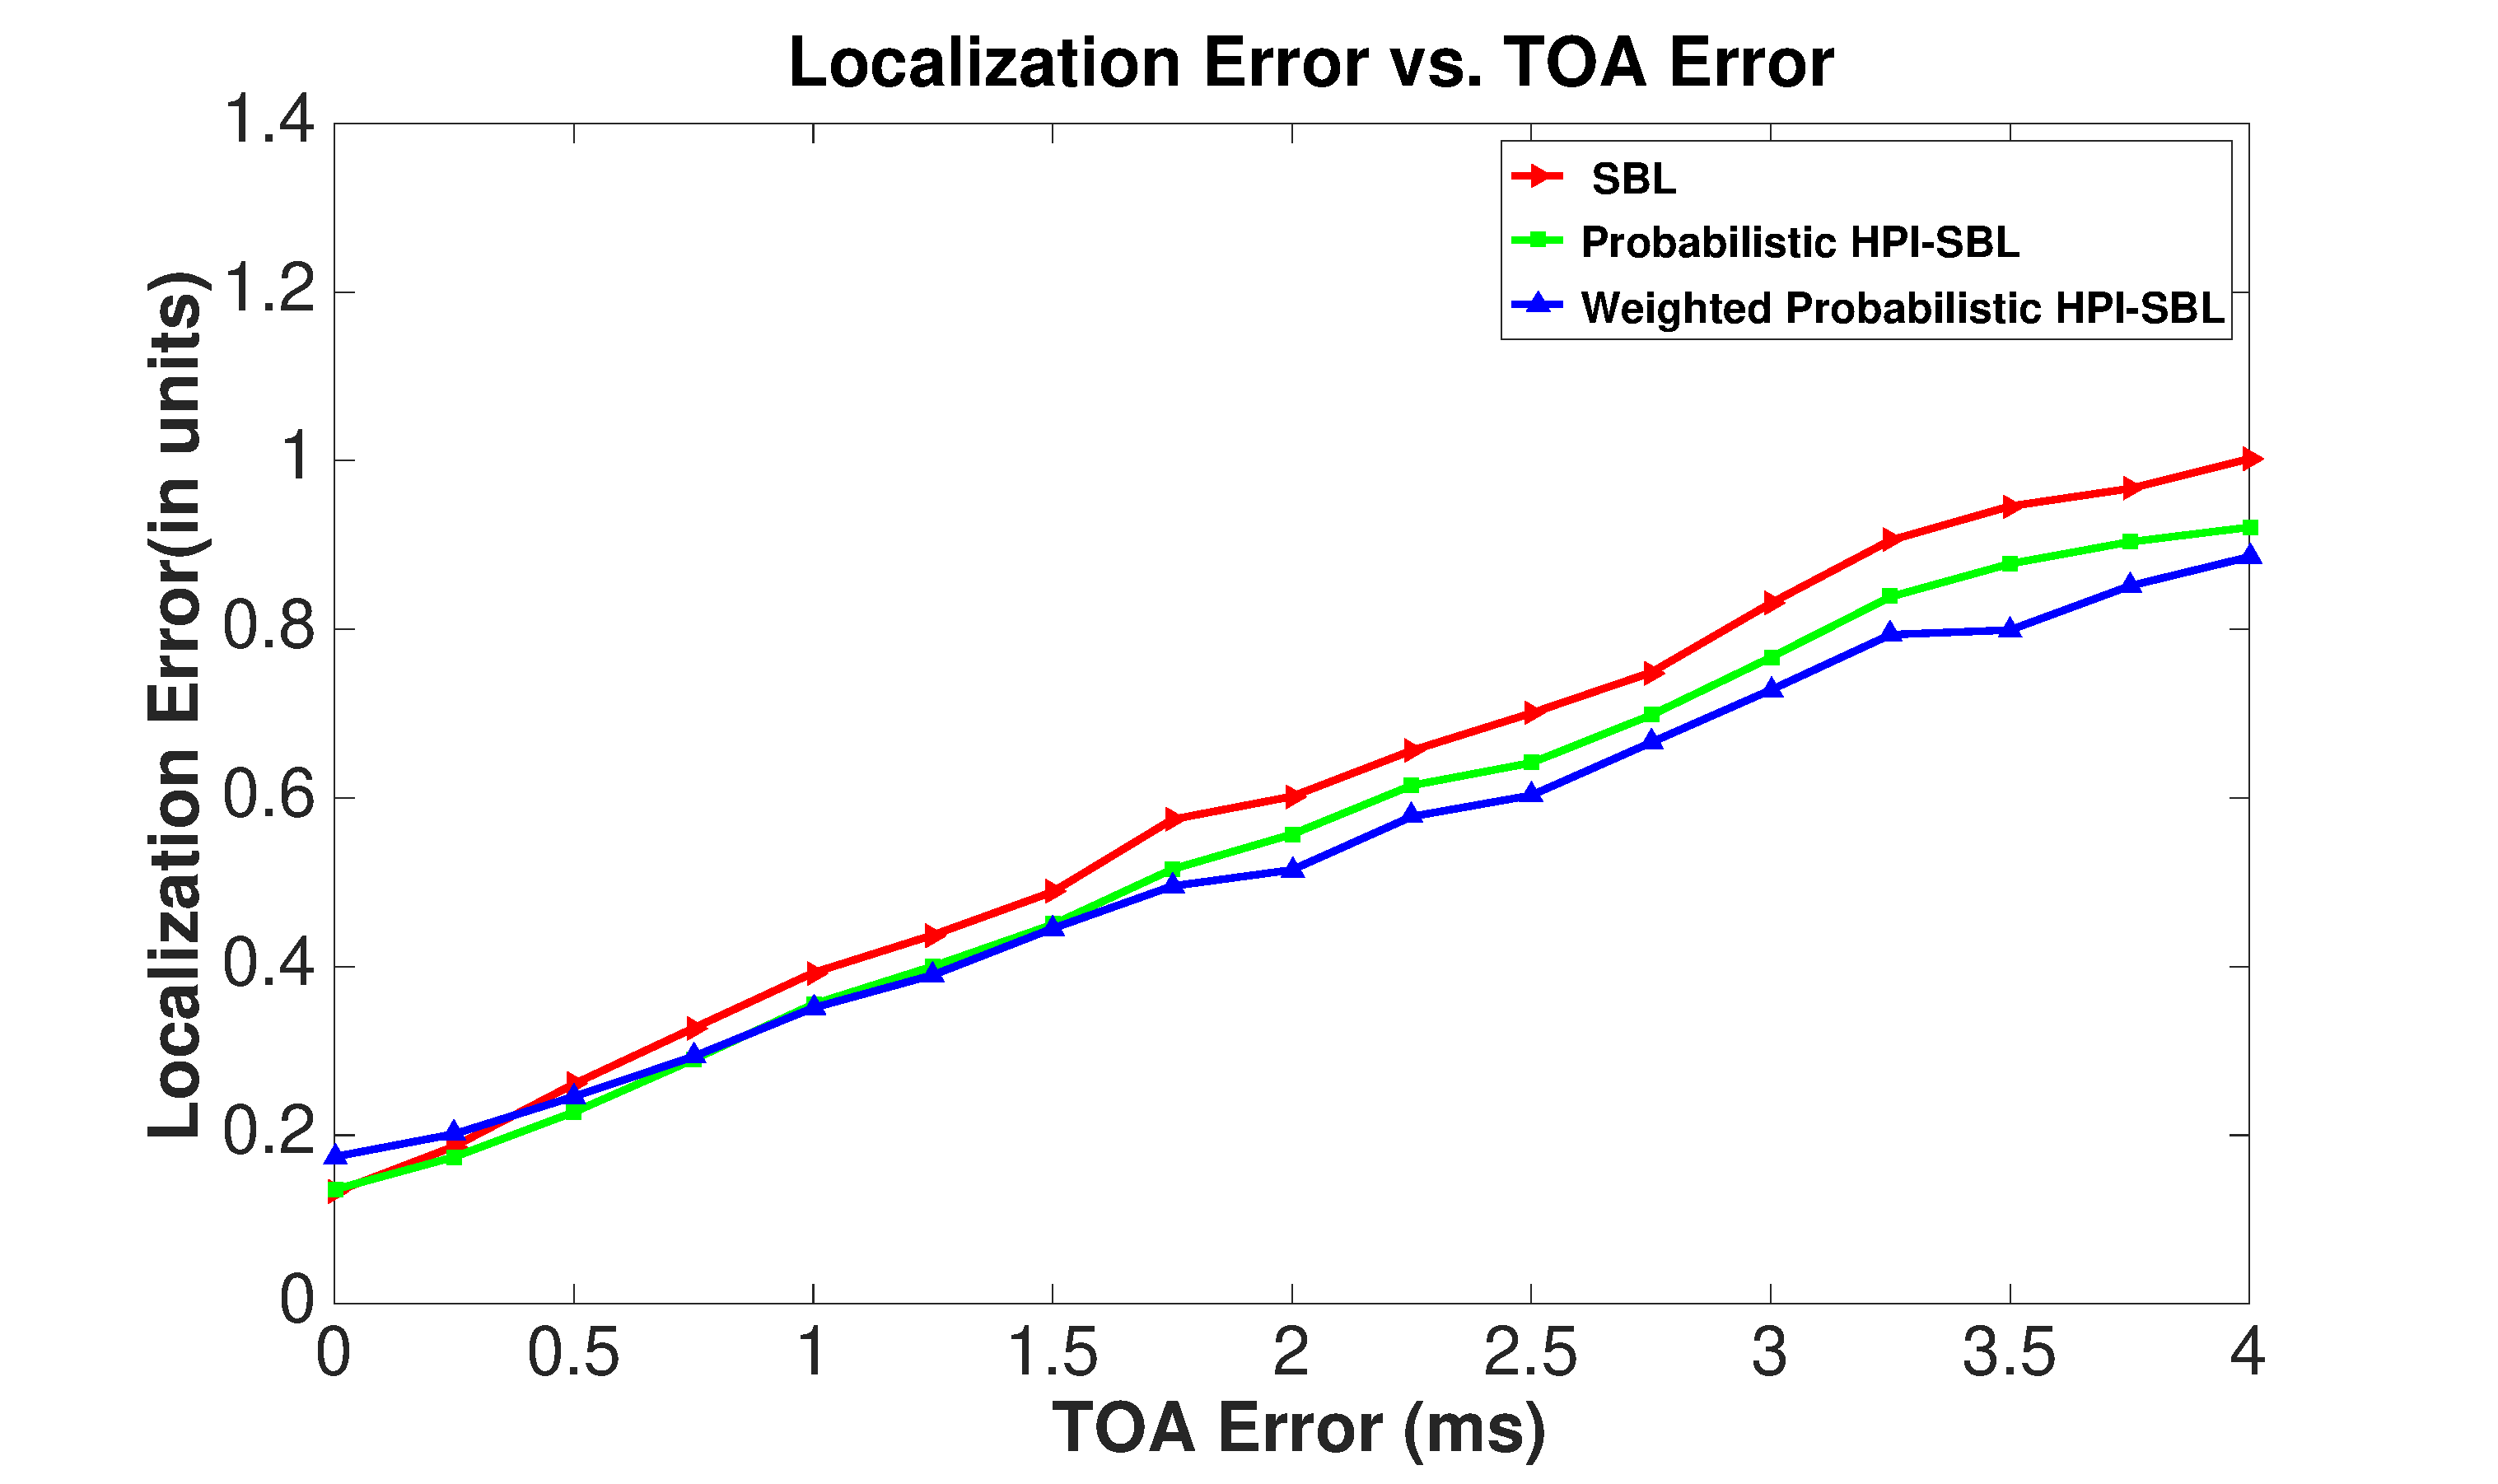
\includegraphics[height=5.0cm,width=7.0cm]{image/TOA.eps}
            \caption{Localization Error vs. TOA Error}
             \vspace{-5mm}
             \label{fig6}
        \end{figure}
		
% \textbf{4) Impact of the probability for P HPI-SBL}
% Time synchronization error maybe also occur flip problem when computing the node sequence in localization system, the impact of time synchronization is similar to TOA measurement error.
% Traditional time synchronization protocol, such as RBS, TPSN, and FTSP, can achieve synchronization with 100ns. 
% Compared with TOA detection error, the effect of time synchronization error is relatively smaller.	
	
  % \begin{figure}[htb]       
            % \centering
			% \vspace{-2mm}
            % 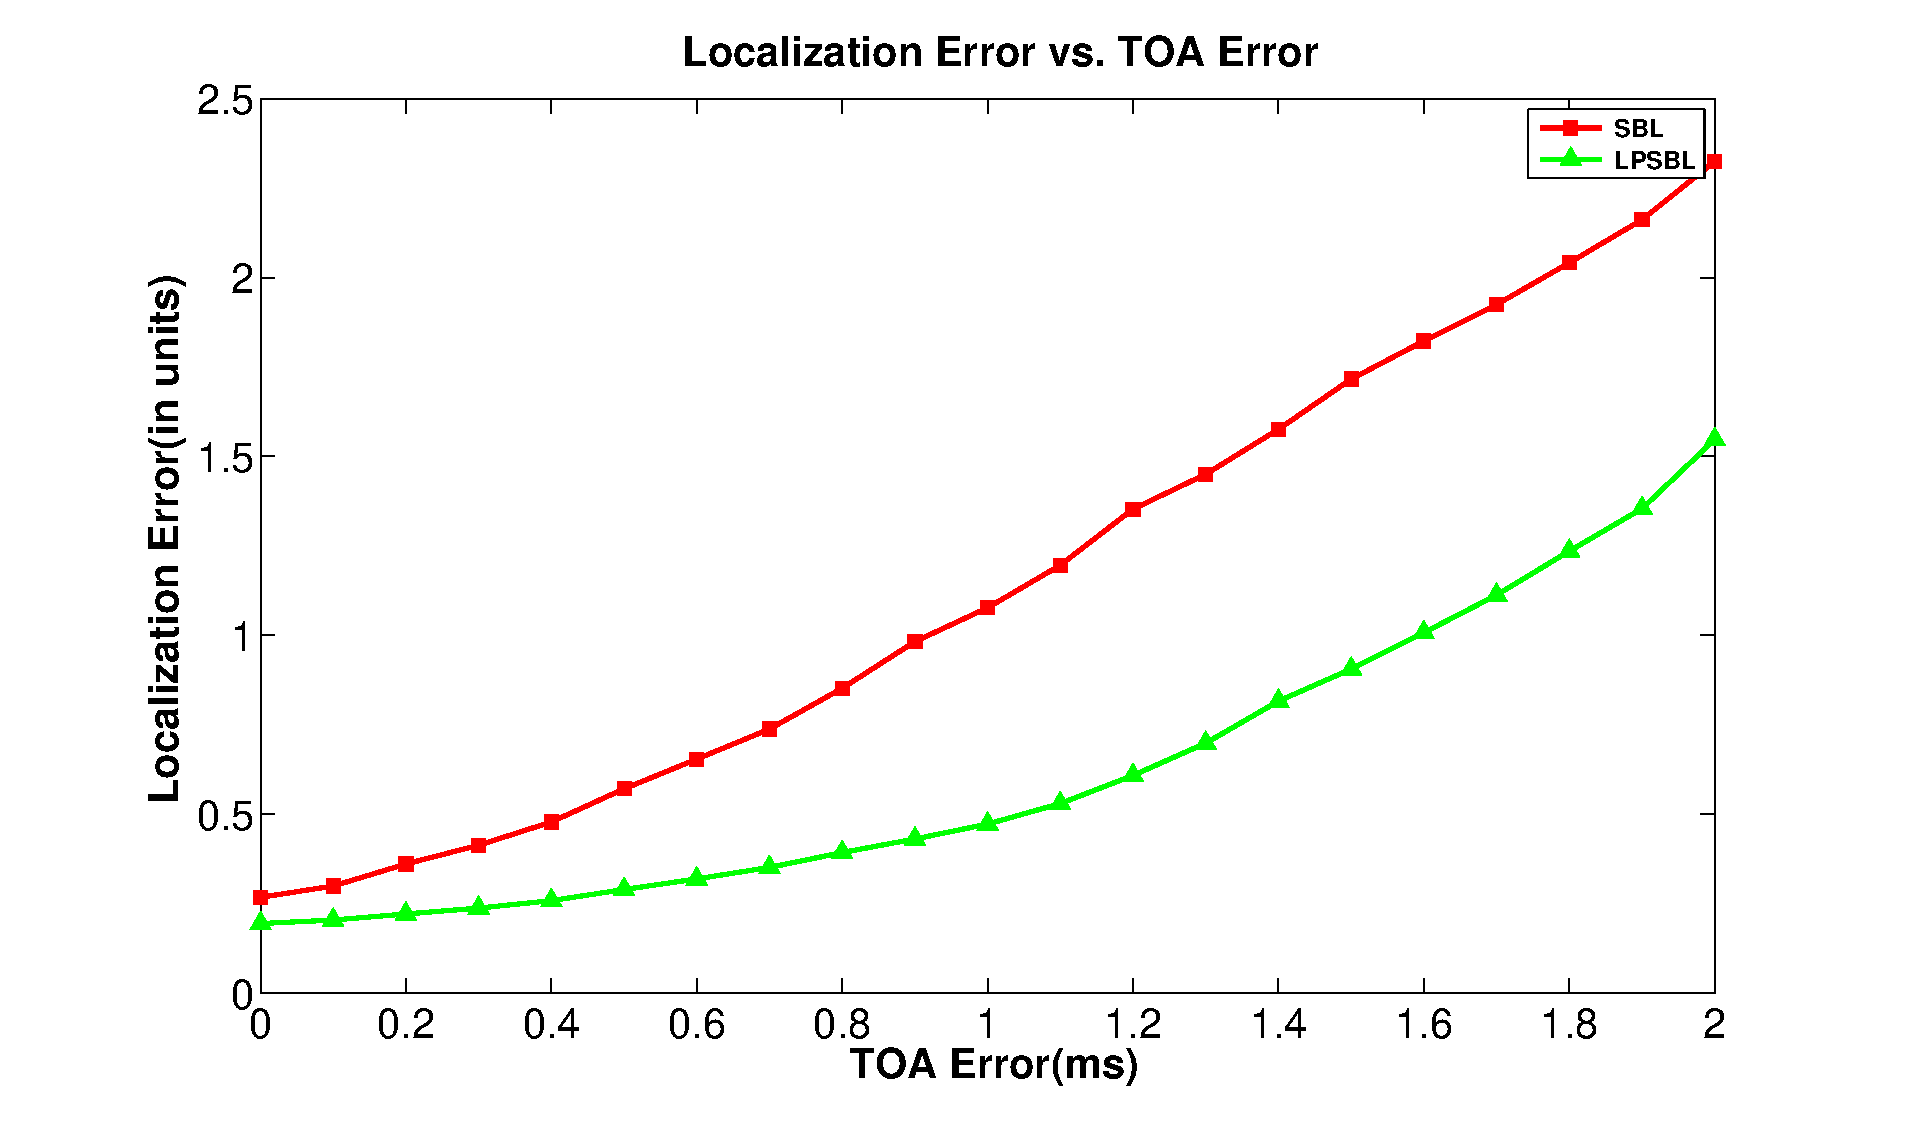
\includegraphics[height=5.0cm,width=7.0cm]{image/fig6.eps}
            % \caption{Localization Error vs. TOA Error}
             % \vspace{-5mm}
             % \label{fig6}
        % \end{figure}



% \textbf{5) Three Weight Scheme P HPI-SBL}

% % 0.5-1   1-0.5   0.5-1-0.5
  % \begin{figure}[htb]       
            % \centering
			% \vspace{-2mm}
            % 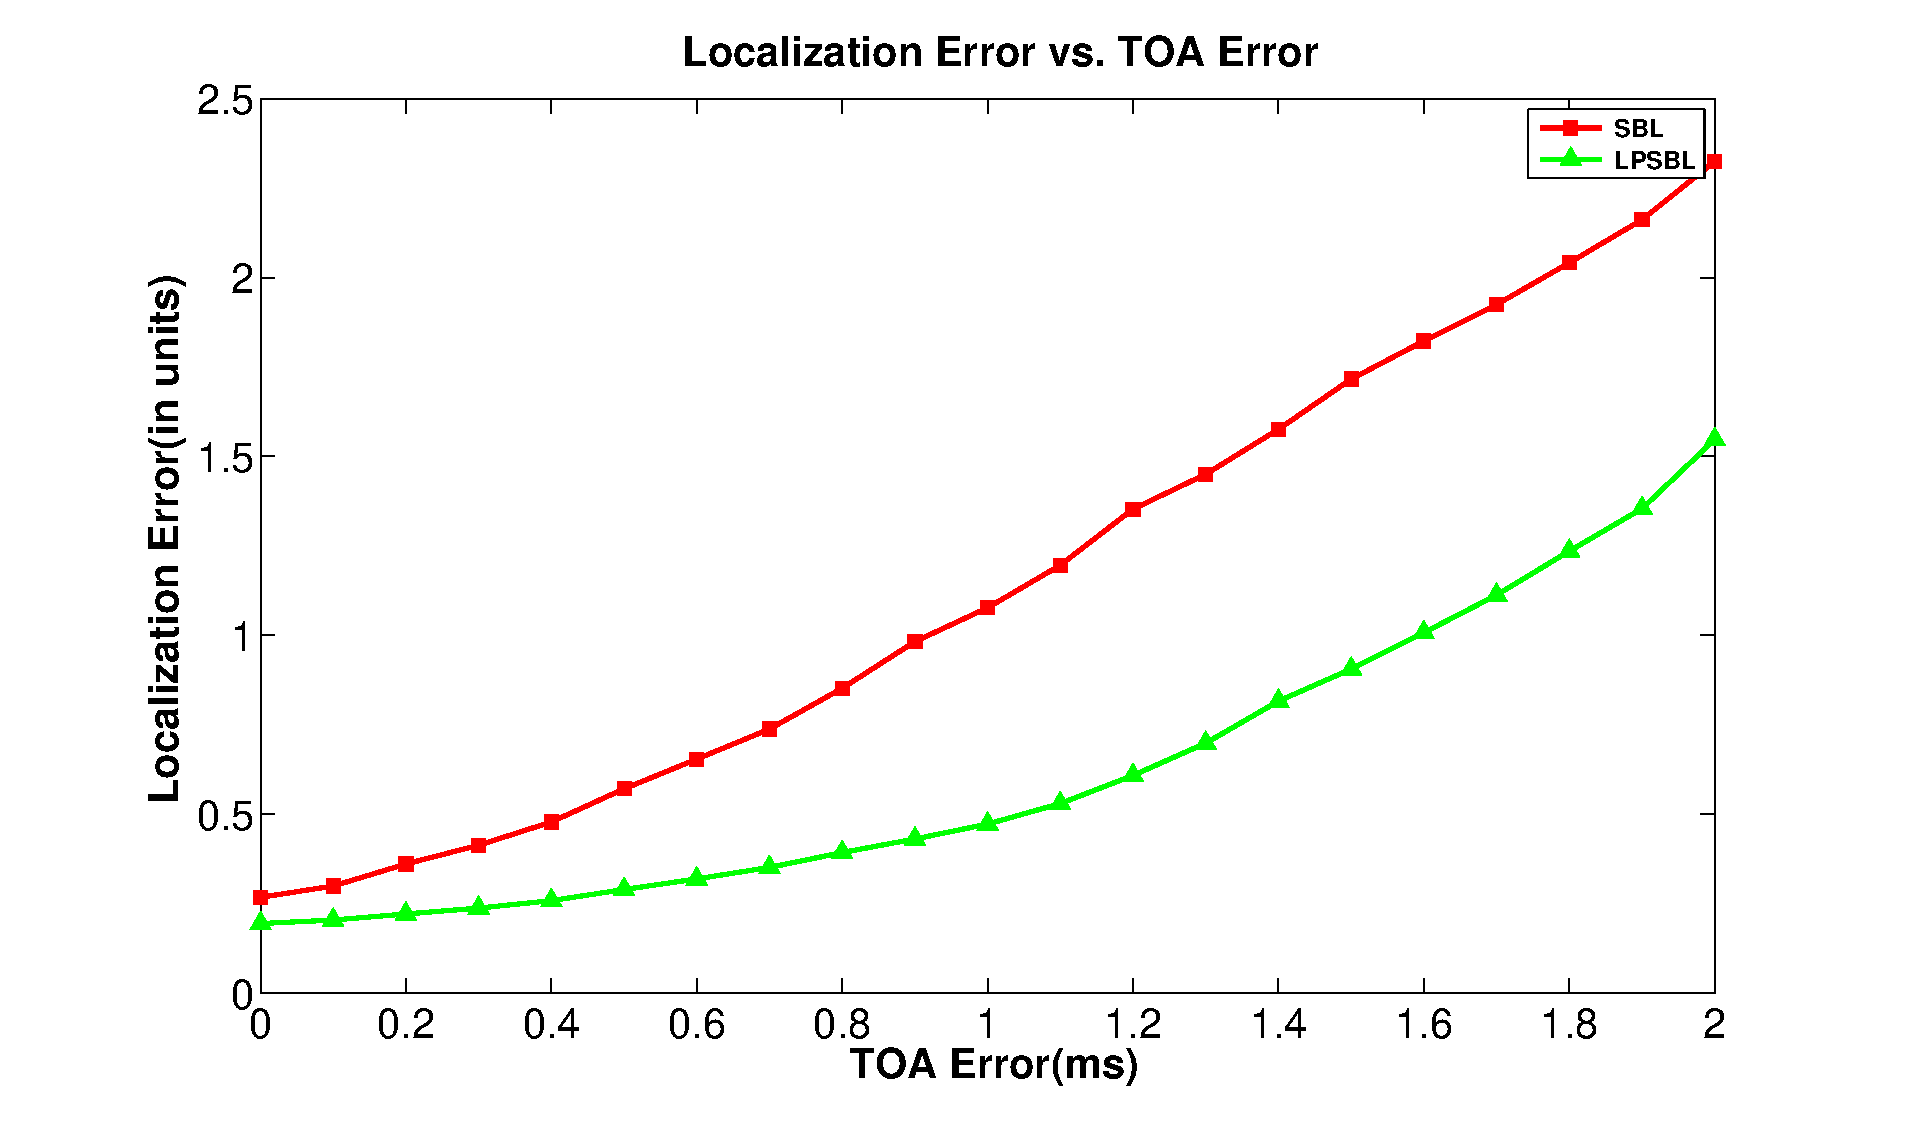
\includegraphics[height=5.0cm,width=7.0cm]{image/fig6.eps}
            % \caption{Localization Error vs. TOA Error}
             % \vspace{-5mm}
             % \label{fig6}
        % \end{figure}

		
 % \textbf{Summary:} From the above simulation results, considering the different factors, 
% including the number of anchors, the node location error and TOA measurement error of the anchors, 
% we can get the conclusion that the proposed HPI-SBL method can achieve better localization performance than SBL method.
% The kernel difference between two methods lies in the way of processing the node sequence.
% By constructing the half-planes from the node sequence, 
% HPI-SBL turns the localization problem into traditional half-plane intersection problem.
% This innovation brings about greatly improved robustness in the localization system.

\subsection{Emulation}


In this section, we reported system implementation of our design based on smartphone arrays.
The 30 smartphones are deployed in a size of 16m$\times$10m space and connected by CISCO CVR328W-K9-CN wireless router.
TPSN protocol is adapted in the proposed HPI-SBL system to realize time synchronization.
In the experiment, smartphones are randomly deployed in the space, and 100 times localization results are shown in Fig.~\ref{fig7}. 
In the figure, blue squares stand for anchor
nodes, red circle squares denote the real position of acoustic sources and black dots are the estimated location by HPI-SBL. 
An arrow origins from the estimated location of each acoustic source and points to its real position. 
As shown in Fig.\ref{fig7}, most of estimated locations are close to the ground truth and the errors between them are very small.
In our experiment, the acoustic sources got localized with average and maximum error of 0.84 feet and 3.91 feet, respectively. Fig.\ref{fig7} tells that
the proposed HPI-SBL successfully accomplishes acoustic source localization with good robustness.


  \begin{figure}[htb]
                  \centering
			    \vspace{-2mm}
            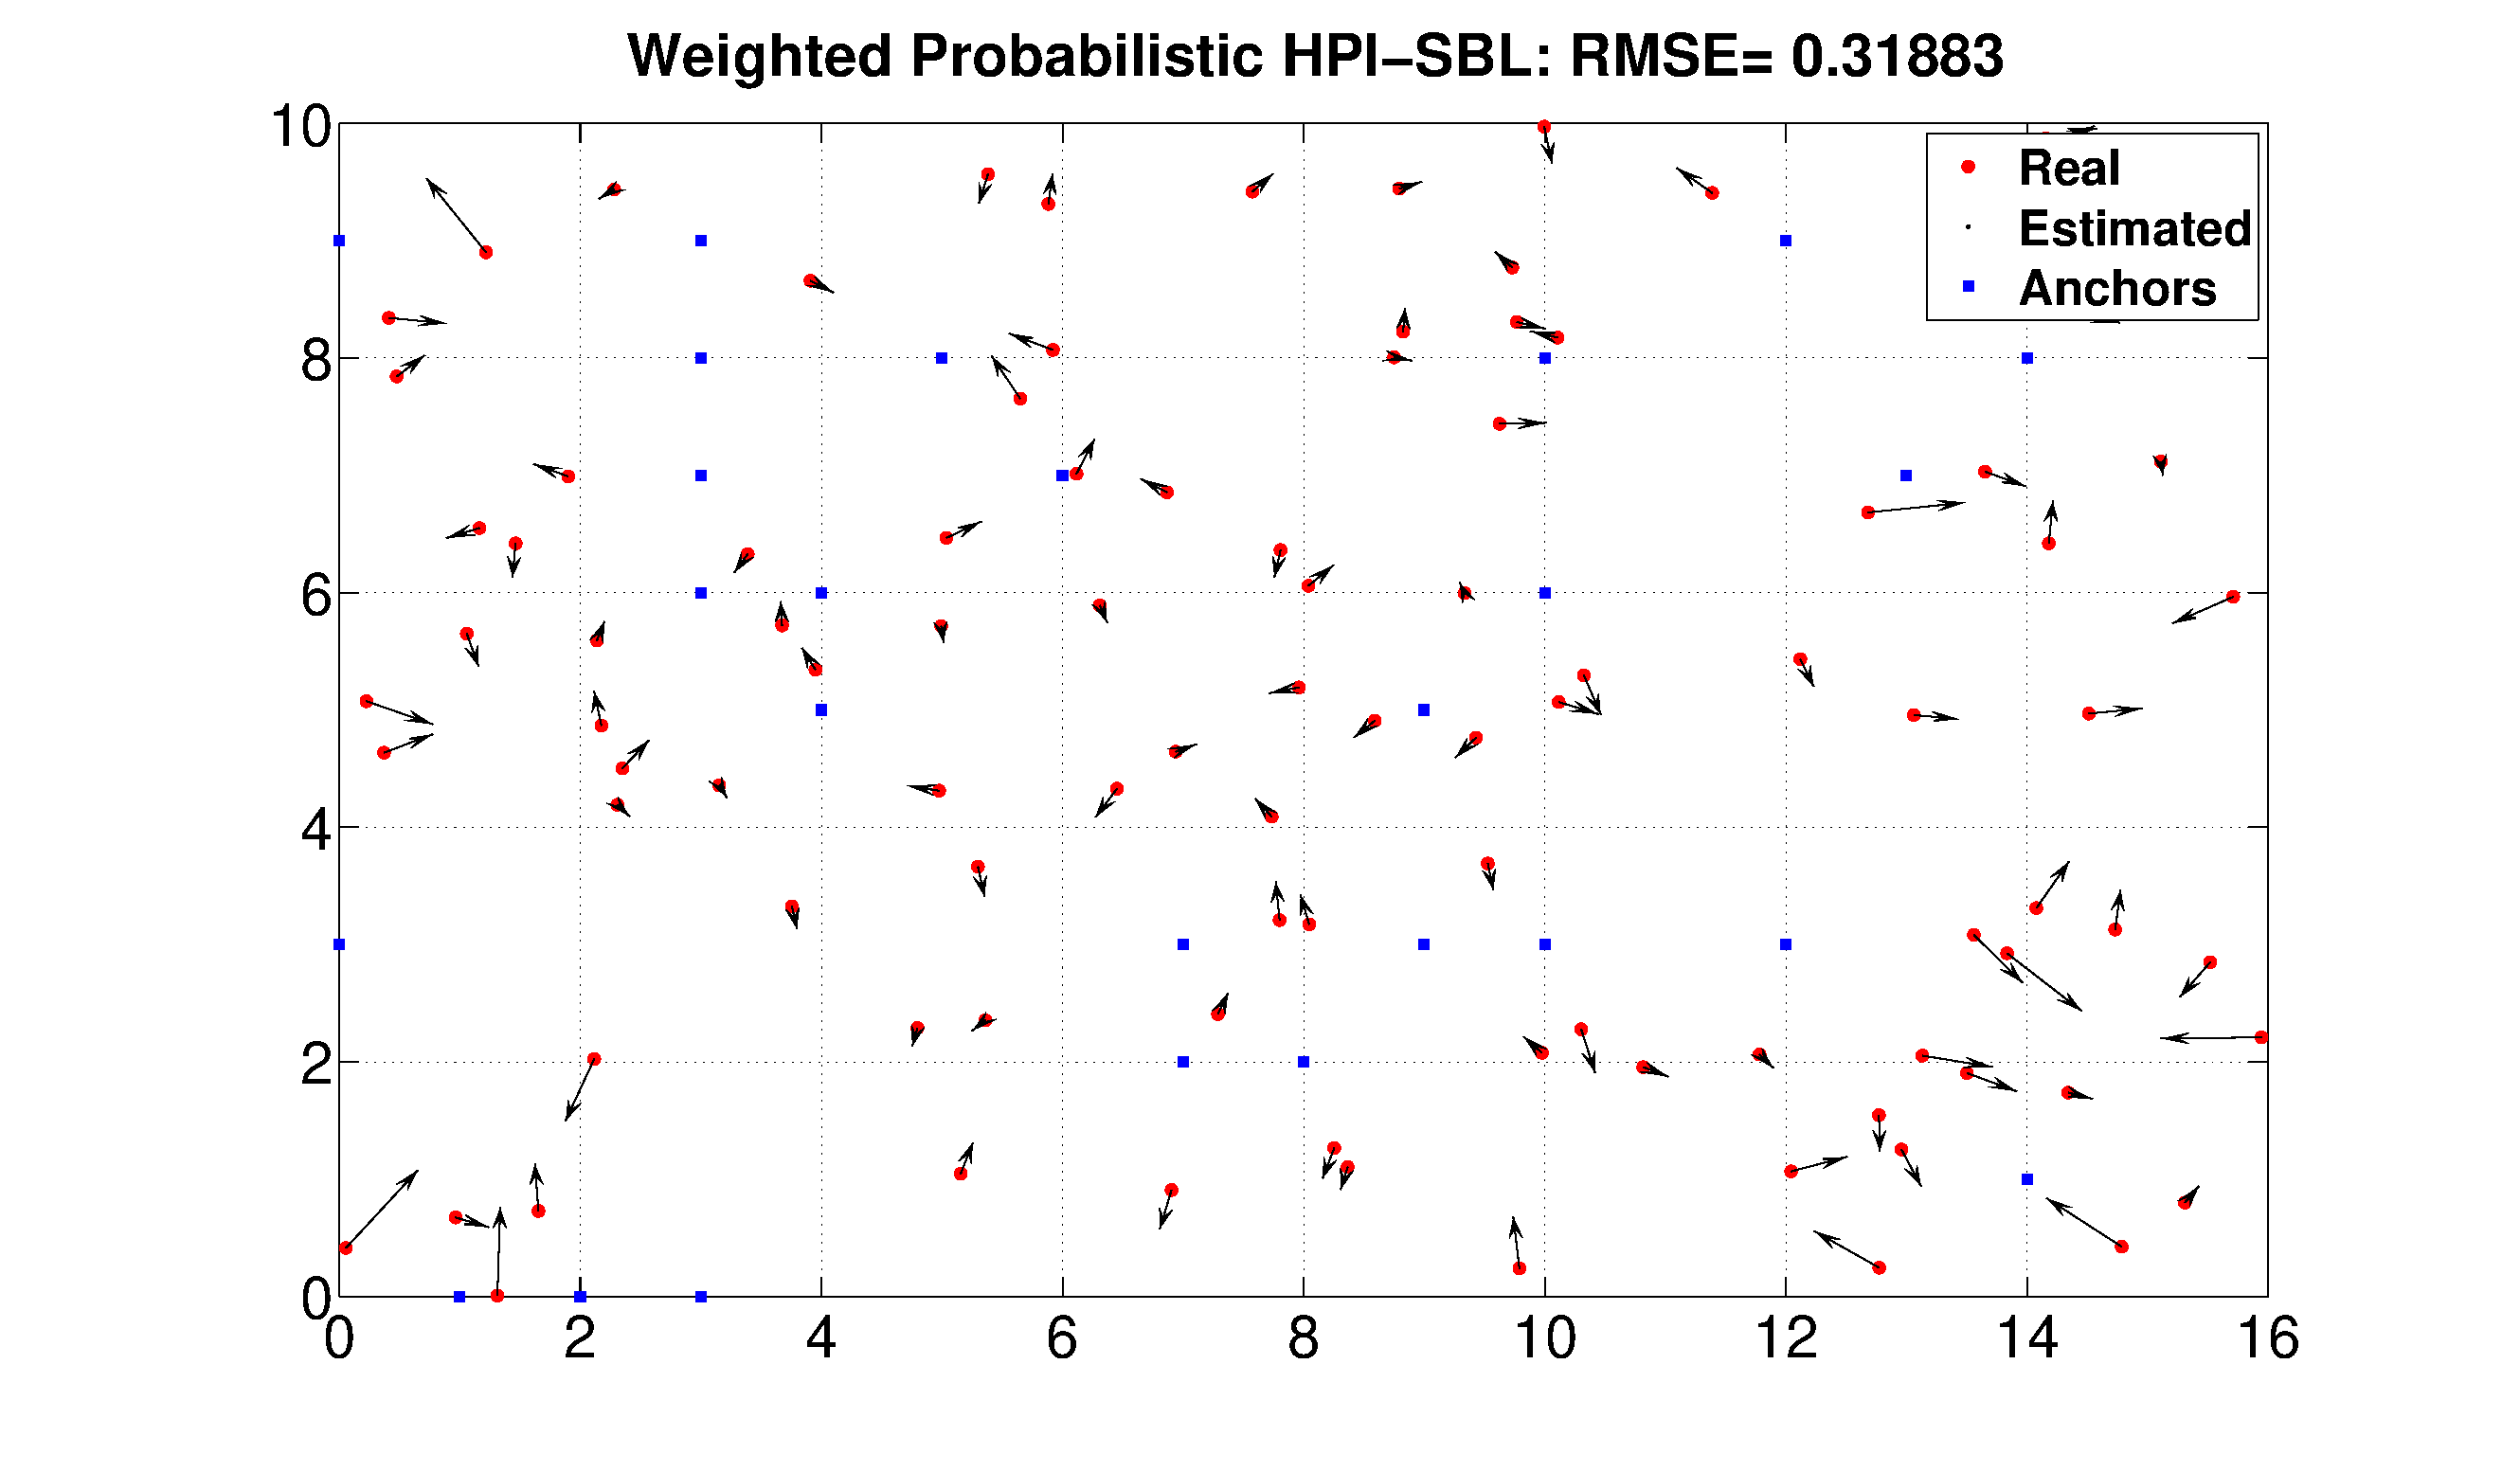
\includegraphics[height=5.0cm,width=7.0cm]{image/testbed.eps}
            \caption{Test-bed localization result of the Weighted Probabilistic HPI-SBL }
             \vspace{-5mm}
             \label{fig7}
        \end{figure}

		
		
\iffalse		
% \begin{figure}[hptb]
% \begin{center}
% \subfigure[Impact of number of anchors]{
% \label{Fig3:3-1}
% \begin{minipage}[t]{0.46\linewidth}
% 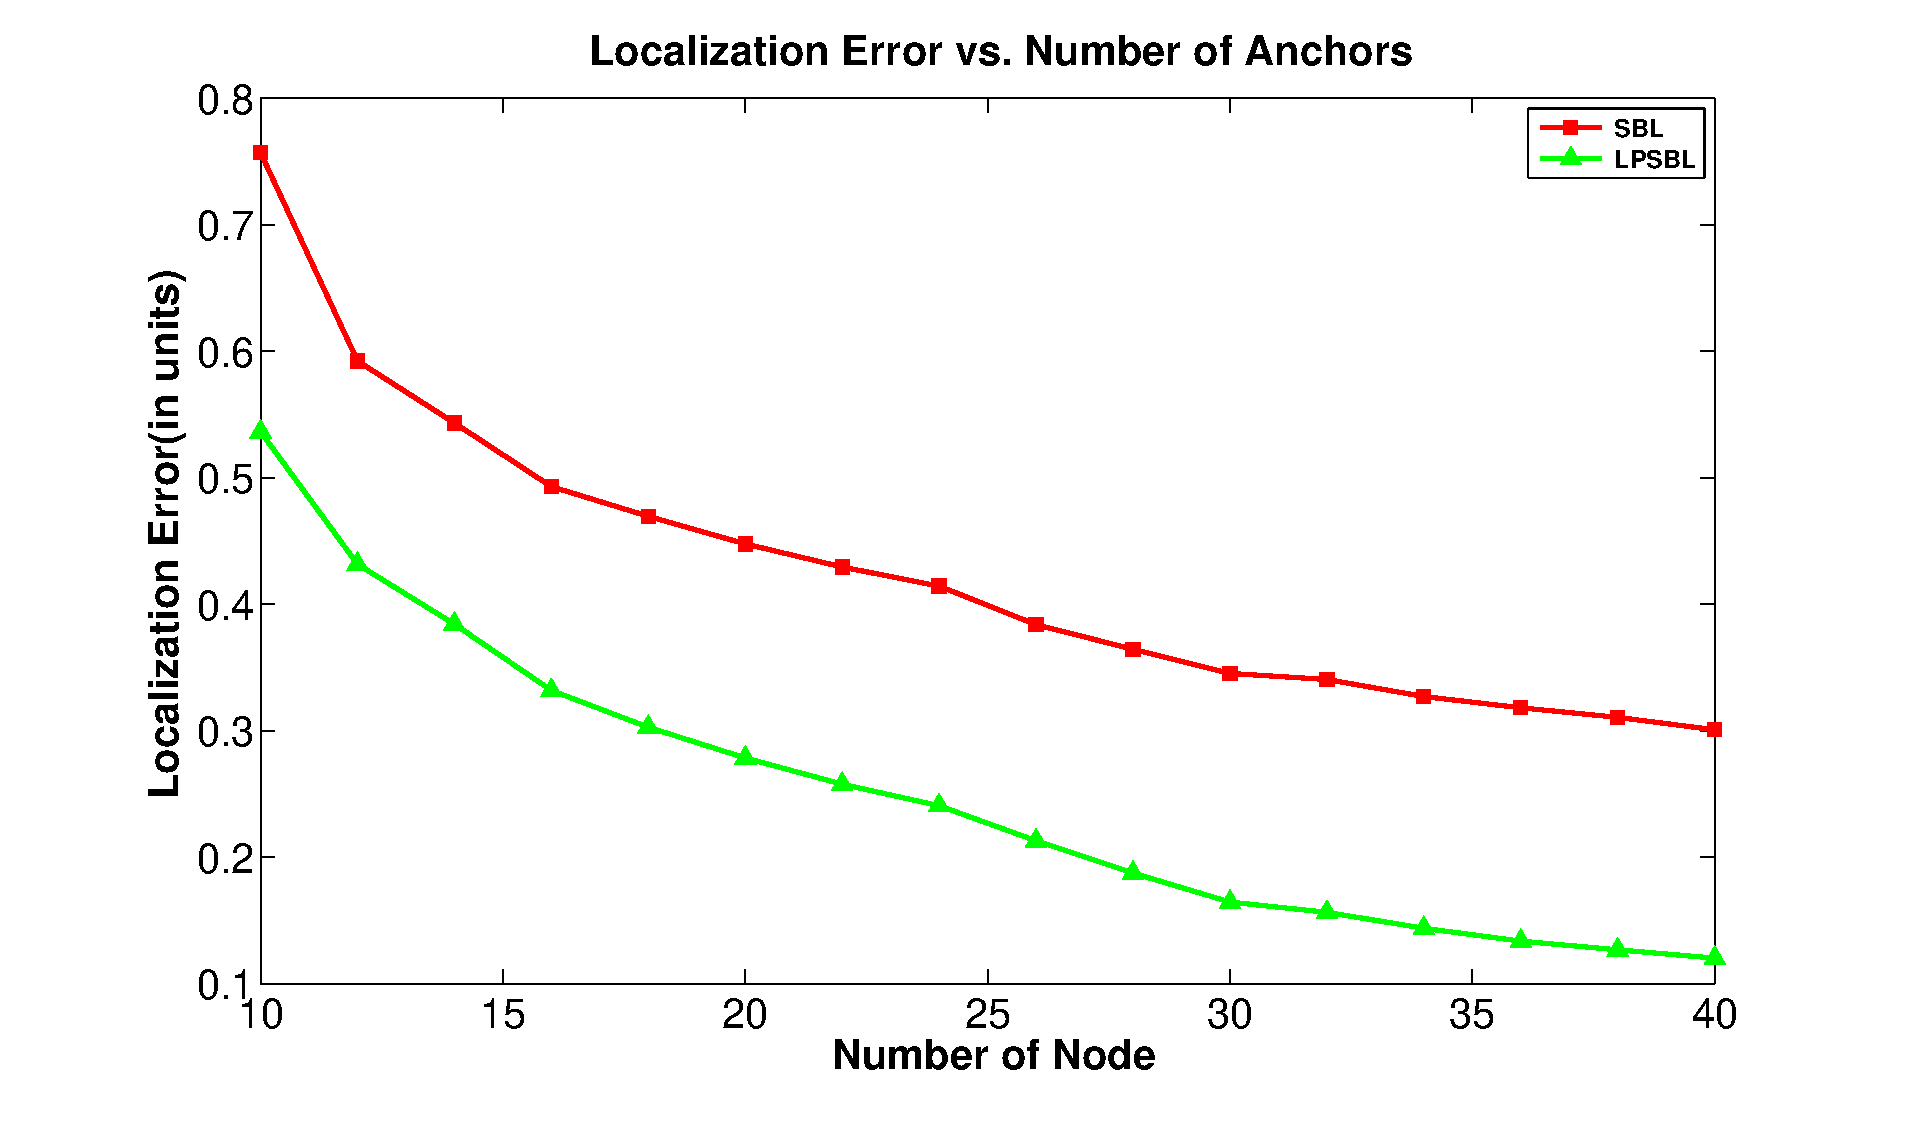
\includegraphics[width=1.150\textwidth]{image/fig4.eps}
% \end{minipage}
% }
% \hspace{-0.1in}
% \subfigure[Impact of node location error]{
% \label{Fig3:3-2}
% \begin{minipage}[t]{0.46\linewidth}
% 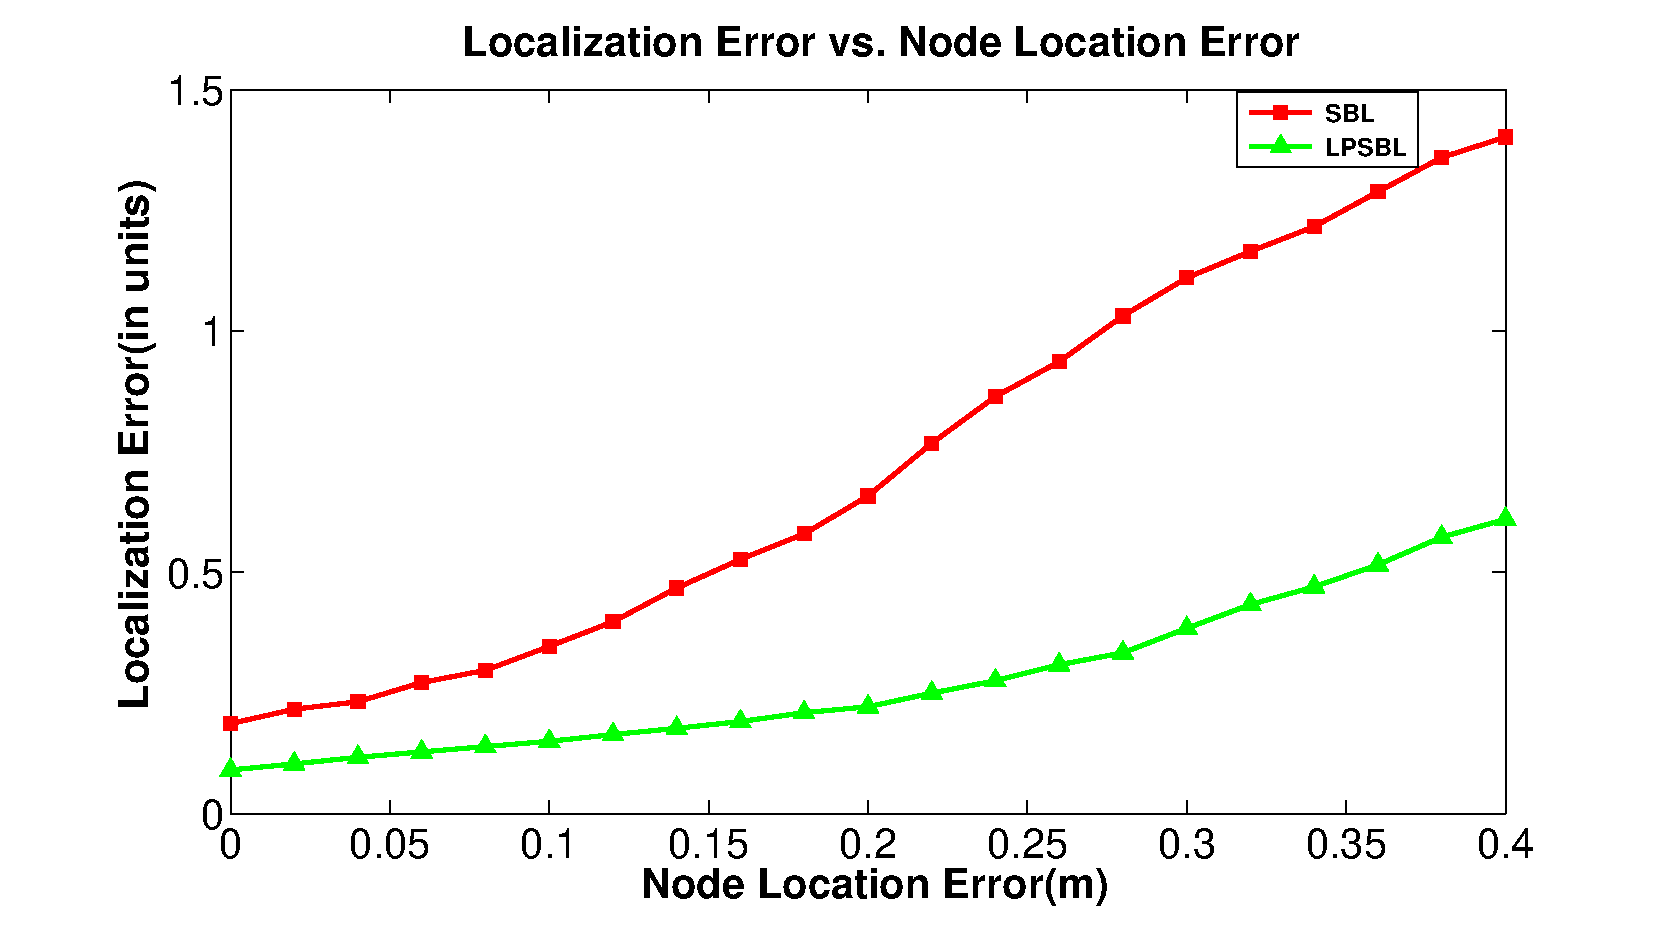
\includegraphics[width=1.150\textwidth]{image/fig5.eps}
% \end{minipage}
% }

% \subfigure[Impact of TOA measurement error]{
% \label{Fig3:3-3}
% \begin{minipage}[t]{0.46\linewidth}
% 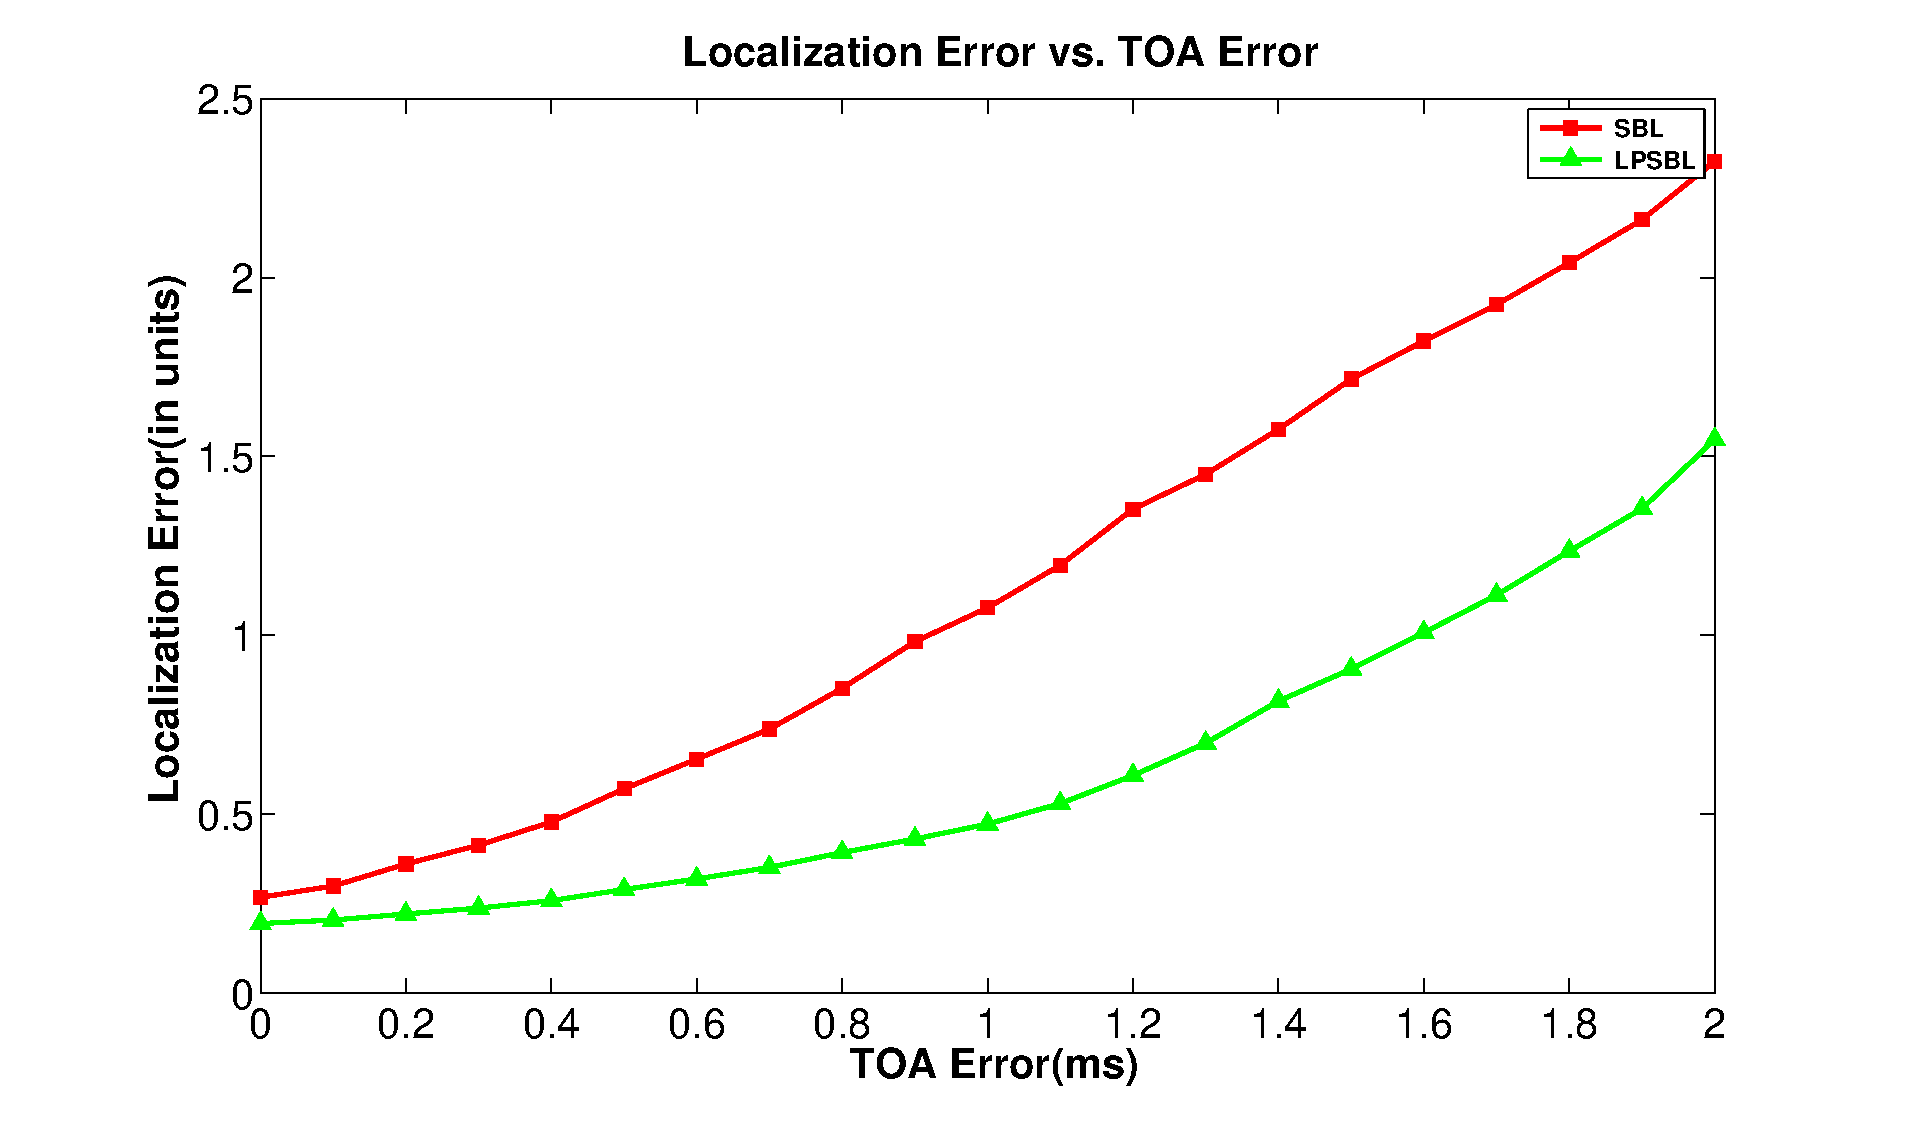
\includegraphics[width=1.150\textwidth]{image/fig6.eps}
% \end{minipage}
% }
% \hspace{-0.1in}
% \subfigure[The results of emulation]{
% \label{Fig3:3-4}
% \begin{minipage}[t]{0.46\linewidth}
% 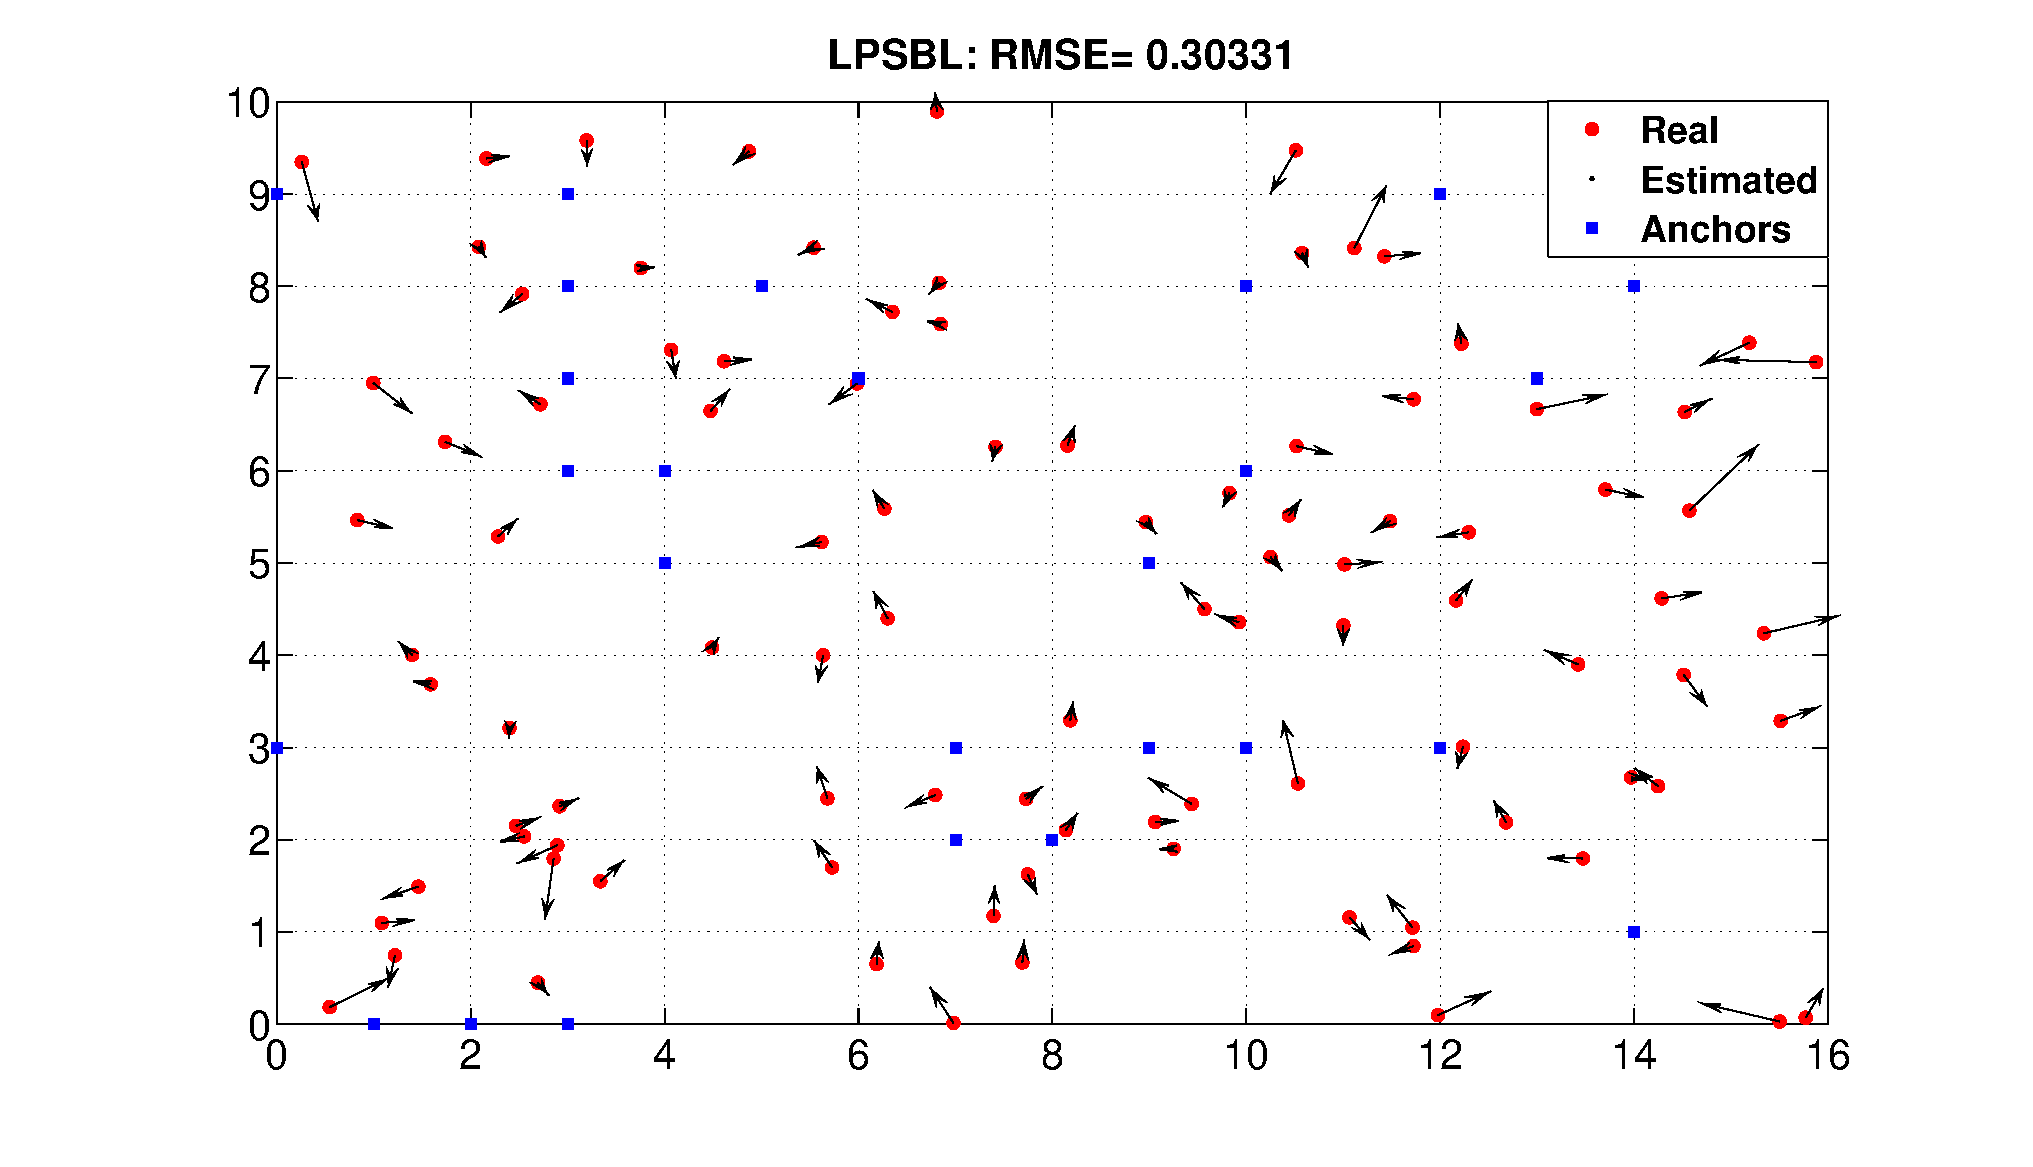
\includegraphics[width=1.150\textwidth]{image/fig7.eps}
% \end{minipage}
% }
% \caption{\label{Fig3:}The results of evaluation.}
% \end{center}
 % \vspace{-5mm}
% \end{figure}
\fi


%%%%%%%%%%%%%%%%%%%%%%%%%%%%%%%%%%%%%%%%%%%%%%%%%


%\section{Related Work}

Acoustic source localization in sensor network is a widely-studied problem. 
In the past few years, there has been a growing interest for spatial distributions of independent (unsynchronized) acoustic sensors, each made of two or more synchronized microphones. Due to space constraints, we can only mention a few directly related works here.
% Omologo, \emph{et al.} \cite{omologo1994acoustic} compute the Steered Response Power maps associated to all the microphone pairs over a spatial grid and then localize the source
% as the peak of the cumulative global map, with overall computational costs that are often too demanding for the application at hand.
% Better computational efficiency is achieved in \cite{cobos2011modified} where the SRP  accommodates a different computation over a coarser grid.
% Alternate approaches based on Least Squares were proposed in \cite{rabinkin1996dsp} with a certain sensitivity to environmental noise;
% and in \cite{do2007real} where a stochastic region contraction of the grid was proposed, adopting a multi-resolution approach.
Wang, \emph{et al.} \cite{wang2003acoustic} described a system having static cluster architecture, the system experienced a problem in that the accuracy decreased when an acoustic source occurred between the clusters.
Chen, \emph{et al.} \cite{chen2004dynamic} showed that nodes in the system did not need to recognize their cluster head, reducing the constraints on deployment of the localization system.
Hu, \emph{et al.} \cite{hu2009design} designed the system based on 2-tier architecture, which experienced cost and deployment problems especially in the very large target area.
Rabbat, \emph{et al.} \cite{rabbat2005robust} proposed a decentralized algorithm based on the distributed ML estimation technique using token ring architecture.
Kim, \emph{et al.} \cite{kim2009locating} proposed to identify the node closest to the acoustic source, based on TOA comparisons between all nodes, thus incurring high communication cost and requiring global synchronization between all sensor nodes.
Lightning is a method proposed in \cite{wang2008lightning} to identify the sensor closest to the acoustic source, also based on expensive broadcasting/flooding.
In previous research on distributed acoustic source localization system, generally each node just has a single element. 
In the past few years, there has been a growing interest for acoustic nodes made of two or more synchronized microphones. 
Aarabi, \emph{et al.} ~\cite{aarabi1900fusion} used 10 dual-microphone arrays distributed in a room and used their data to locate three speakers.
Wu, \emph{et al.} ~\cite{wu2012fusion} used three dual-microphone arrays to locate two sound sources in a distributed way in which only the local DOA estimates are communicated among arrays.
Canclini, \emph{et al.}\cite{canclini2013acoustic,Canclini2015} proposed a method for localizing an acoustic source with distributed microphone networks based on TDOA between microphones of the same sensor.

Most of the existing acoustic source localization methods in sensor networks are based on range-based measurement.
In contrast, our work is a range-free method and shown to be robust to the errors of node locations and the errors of measurements.
There have existed some research on range-free localization method.
Yedavalli, \emph{et al.} ~\cite{yedavalli2008sequence} proposed a Sequence-Based Localization (SBL) method in WSN. 
The heart of SBL is the division of a 2D localization space into distinct regions by the perpendicular bisectors of lines joining pairs of reference nodes (nodes with known locations).
%Each distinct region formed in this manner can be uniquely identified by a location sequence that represents the distance ranks of reference nodes to that region. 
%The unknown node first determines its own location sequence based on the measurement between itself and the reference nodes, then searches through the location sequence table to determine its location.
In their earlier work \cite{yedavalli2005ecolocation}, Ecolocation used location constraints for robust localization.
%A location constraint is a relationship between the distances of two reference nodes from the unknown node that determines its proximity to either
%reference nodes. Location constraints can be graphically represented by perpendicular bisectors
%between reference nodes, and each location sequence can be written as a set of location constraints.
%Thus, the location constraint set is also unique to each region in the arrangement.
Chakrabarty, \emph{et al.} \cite{chakrabarty2002grid} and Ray, \emph{et al.} \cite{ray2004robust} used identity codes to determine the location of sensor nodes in grid and nongrid sensor fields, respectively. 
He, \emph{et al.} \cite{he2003range} proposed an RF-based localization technique in which the unknown node location is determined by the intersection of all triangles,
formed by reference nodes, that are likely to bound it. The unknown node determines its existence inside a triangle by
comparing its measured RSS values to that of its neighbors to detect a trend in RSS values in any particular direction
This technique depends on the weak assumption that signal strength decreases monotonically with distance, which is not true in real-world scenarios.
Zhong, \emph{et al.} \cite{zhong2009tracking} converted the original tracking problem to the problem of finding the shortest path in a graph, which is equivalent to optimal matching of a series of node sequences. 
Zhong, \emph{et al.} \cite{zhong2011rsd} introduced a proximity metric called RSD to capture the distance relationships among 1-hop neighboring nodes in a range-free manner. 
Guo, \emph{et al.} \cite{guo2014detecting}  proposed a novel method to detect nodes with data faults by ranking the nodes based on their sensing
readings from the event.
Shu, \emph{et al.} \cite{shu2015toc}  proposed a novel localization design that utilizes the unique Time of Charge (TOC) sequences among wireless rechargeable sensors.
Zhong, \emph{et al.} \cite{zhong2012wireless} presented a Multi-Sequence Positioning (MSP) method for  sensor node localization by processing multiple one-dimensional node sequences.
Yang, \emph{et al.} \cite{yang2013freeloc} used the relative relationship information between RSS values as the fingerprint data in the Wi-Fi indoor positioning system.


%localize nodes based on their connectivity information or simple sensing of their relative positions.

%rang free ??
%Q. Xu, A. Gerber, Z. M. Mao, and J. Pang. 2011. AccuLoc: Practical localization of performance measurements in 3g networks. In ACM MobiSys.

%rang free ?? L. Doherty, K. S. J. Pister, and L. El Ghaoui. 2001. Convex position estimation in wireless sensor networks.In IEEE INFOCOM.

\section{Conclusions}

In this paper, we presented a simple and novel localization technique based on half-plane intersection, HPI-SBL. 
The reference nodes sequence is computed by using TOA measurements of acoustic signals between the acoustic source and the reference nodes.
The half-planes are constructed by processing the node sequence, then turn the localization problem into half-plane intersection problem. 
Since our system runs on COTS smartphones and supports spontaneous setup, 
it has potential to enable a wide range of distributed acoustic localization system. 
 Besides the basic design,  robust HPI-SBL is proposed for further enhancing system robustness.
 Our system is verified and evaluated through analysis, extensive simulation as well as the test-bed experimentation.
 The test results have shown that the proposed method can effectively implement aoustic source localization with ad-hoc smartphone array.
 Our next step is to study the distributed localization method for ad-hoc smartphone array.
%Another future work is that further mining the information embedded in the node sequence to improve the robustness of localization system.

% \section{Acknowledge}

% This work is supported by Natural Science Foundation of China (Grants No. 61272524 and No.61202443) and the Fundamental Research Funds for the Central Universities (Grants No.DUT15QY05 and No.DUT15QY51). 
% This work is also supported by Specialized Research Fund for the Doctoral Program of Higher Education (Grant No. 20120041120049).


	
	%\vfill\pagebreak
	
	
	\bibliographystyle{IEEEbib}
	\bibliography{Main}
	
\end{document}











